\section{ESTUDOS DE CASO}\label{sec:4ec-estudosdecaso}

Ao longo do Capítulo~\ref{sec:3deap-implagentes} foram abordados os principais aspectos da implementação da PG, através da biblioteca DEAP. Principalmente, a implementação da: representação e inicialização de indivíduos, avaliação, seleção e alteração dos membros da população. O que se espera de cada iteração da programação genética são valores crescentes de aptidão.

Diversos problemas são abordados ao longo deste capítulo. Para cada caso, uma tabela é apresentada com os principais parâmetros do ciclo evolucionário. Além disso, alguns aspectos adicionais particulares a cada caso serão incluídos, como, por exemplo, a função de avaliação.

Abaixo, é incluída uma breve explicação de cada parâmetro e sua implementação.

\begin{itemize}[label=\raisebox{0.25ex}{\tiny$\bullet$}]
	\item \textit{Tamanho da população ($tam\_pop$)}: O número de indivíduos da população.
	\item \textit{Probabilidade de cruzamento ($pb\_cx$)}: probabilidade de que a operação escolhida seja cruzamento.
	\item \textit{Probabilidade de mutação ($pb\_mut$)}: probabilidade de que a operação escolhida seja mutação.
	\item \textit{Número de gerações ($n\_geracoes$)}: quantas vezes o ciclo de avaliação, seleção e variação da população ocorrerá.
	\item \textit{Tipo de aptidão ($tipo\_apt$)}: define se deseja-se minimizar ou maximizar uma medida de aptidão. Ex: $1$ indica que o objetivo é maximizar a função de aptidão. O valor $-1$ aponta o contrário.
	\item \textit{Número de entradas ($n\_entradas$)}: número de variáveis de estado.
	\item \textit{Faixa para a constante efêmera ($faixa\_cst$)}: valor mínimo e máximo que limitam os valores possíveis para a variável terminal de valor aleatório.
	\item \textit{Número de simulações ($n\_episodios$)}: número de episódios (simulações) para avaliação de cada indivíduo.
	\item \textit{Tamanho do torneio de aptidão ($camp\_apt$)}: número de indivíduos que irão compor o torneio de aptidão.
	\item \textit{Tamanho do torneio de comprimento ($camp\_d$)}: pressão de seleção sobre indivíduos aspirantes ao torneio de aptidão (valor entre $1$ e $2$).
	\item \textit{Operações}: operações que compõe os nós não-terminais da árvore.
	\item \textit{Comprimento mínimo e máximo de inicialização ($d\_min$, $d\_max$)}: comprimentos mínimos e máximos possíveis dos indivíduos inicializados.
	\item \textit{Comprimento máximo de mutação ($max\_d\_mut$)}: A função geradora de expressões será diferente para a mutação. O comprimento mínimo será sempre zero, entretanto o máximo irá variar, dependendo da complexidade da solução esperada.
	\item \textit{Limite de comprimento dos indivíduos ($limite\_d$)}: comprimento máximo dos indivíduos gerados através das operações de mutação e cruzamento (controle de bloat).
\end{itemize}

As seguintes estatísticas relacionadas à evolução da população e à execução do programa são obtidas:

\begin{enumerate}[label=\alph*)]
	\item \underline{Em relação à aptidão: } este é o principal parâmetro a ser observado e a expectativa é que essa medida aumente ao longo do tempo. Ao longo de cada geração, as seguintes medidas de aptidão serão obtidas.
	\begin{itemize}[label=\raisebox{0.25ex}{\tiny$\bullet$}]
		\item \textit{Mínimo: } valor de aptidão do indivíduo de pior desempenho.
		\item \textit{Máximo: } valor de aptidão do indivíduo de melhor desempenho.
		\item \textit{Média: } valor médio de aptidão da população.
	\end{itemize}
	\item \underline{Em relação ao comprimento: } Medida que indica o maior comprimento (ou profundidade) da árvore, conforme aponta a Figura \ref{fig:3deap-profundidade}. As medidas relacionadas a esse parâmetro, ao longo de cada geração, serão:
	\begin{itemize}[label=\raisebox{0.25ex}{\tiny$\bullet$}]
		\item \textit{Mínimo: } valor mínimo de profundidade encontrado na geração.
		\item \textit{Máximo: } valor máximo de profundidade encontrado na geração.
		\item \textit{Média: } valor médio de profundidade da população.
	\end{itemize}
	\item \underline{Em relação à complexidade: } esta medida indica o número total de nós em um indivíduo (operadores e variáveis terminais), em cada geração.
	\begin{itemize}[label=\raisebox{0.25ex}{\tiny$\bullet$}]
		\item \textit{Mínimo: } menor número de nós encontrado em um indivíduo na população.
		\item \textit{Máximo: } maior número de nós encontrado em um indivíduo na população.
		\item \textit{Média: } número médio de nós da população, para cada indivíduo.
	\end{itemize}
\end{enumerate}

Foi realizada uma comparação da PG com dois algoritmos de aprendizagem profunda por reforço: \textbf{DQN} (\textit{Deep Q-Learning}) \cite{silver2013dqn} e \textbf{DDPG} (\textit{Deep Deterministic Policy Gradient}) \cite{lili2015ddpg}.

\subsection{Pêndulo Invertido}\label{ssec:4ec-cartpole}

O problema básico que foi escolhido para servir de exemplo, para a aplicação da PG, foi o pêndulo invertido. Os parâmetros utilizados apresentam-se na Tabela \ref{tab:4ec-param-cartpole}.

\begin{table}[H]
	\centering
	\begin{tabular}{l|l} \toprule
		{Parâmetro} & {Valor} \\ \midrule
		{Tamanho da População} & {500} \\
		{Probabilidade de Cruzamento} & {0,75} \\
		{Probabilidade de Mutação} & {0,05} \\
		{Número de Gerações} & {15} \\
		{Número de Entradas} & {4} \\
		{Faixa para Constante Efêmera} & {(-1, 1)} \\
		{Número de Simulações} & {10} \\
		{Tamanho do Torneio de Aptidão} & {6} \\
		{Tamanho do Torneio de Comprimento} & {1,2} \\
		{Operações} & {$+,\,-,\,\times,\,\div,\,\sqrt{},\,\sin,\,>$, sgn} \\
		{Comprimento Mínimo e Máximo de Inicialização} & {(1, 3)} \\
		{Comprimento Máximo de Mutação} & {5} \\
		{Limite de Comprimento dos Indivíduos} & {17} \\
		\bottomrule
	\end{tabular}
	\caption{Parâmetros da PG para o problema do pêndulo invertido.}\label{tab:4ec-param-cartpole}
\end{table}

A função de cálculo de aptidão, é tal como descrita na Equação \ref{eq:3deap-calcaptidaototpendinv}, isto é, a média do tempo total em que o bastão permanece equilibrado, em vários episódios, respeitando os limites estabelecidos na Tabela \ref{tab:2gym-observacao}. Já que a simulação tem uma duração limite de 500 passos de tempo, a aptidão máxima possível é 500. Como as condições iniciais são aleatórias, a medida de desempenho é realizada através da aptidão média obtida em vários episódios (parâmetro representado pelo número de simulações).

Utilizando os dados da Tabela \ref{tab:4ec-param-cartpole}, o algoritmo foi executado 10 vezes em sequência e a média das estatísticas foram obtidas. O algoritmo completo encontra-se no apêndice \ref{apendice:codigos}.

\begin{figure}[H]
	\centering
	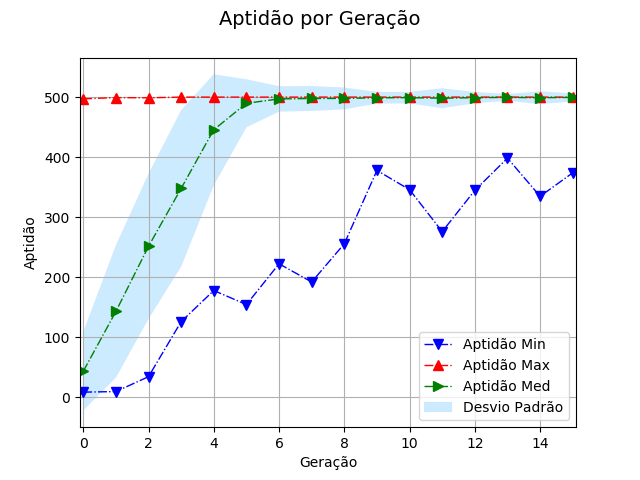
\includegraphics[width=0.8\textwidth]{02_desenvolvimento/04_EC_Fig_CartpoleAptGer.png}
	\caption{Média da aptidão de todos os indivíduos por geração (verde). Valor máximo de aptidão observado em cada geração (vermelho). Menor aptidão observada em cada geração (azul).}
	\label{fig:4ec-cartpoleaptger}
\end{figure}

Observa-se no gráfico da Figura \ref{fig:4ec-cartpoleaptger}, que na primeira geração alguns indivíduos já são capazes de obter a aptidão máxima. Isto se deve, em parte, ao grande número de indivíduos (500) gerados aleatoriamente, o que funciona, de certa forma, como uma busca exaustiva.

Entretanto, ainda é possível observar o aumento da aptidão média e mínima ao longo das gerações. O gráfico da Figura \ref{fig:4ec-cartpoleapthist} mostra o número de indivíduos que atingiram uma determinada faixa de aptidão, em algumas geração.

\begin{figure}[H]
	\centering
	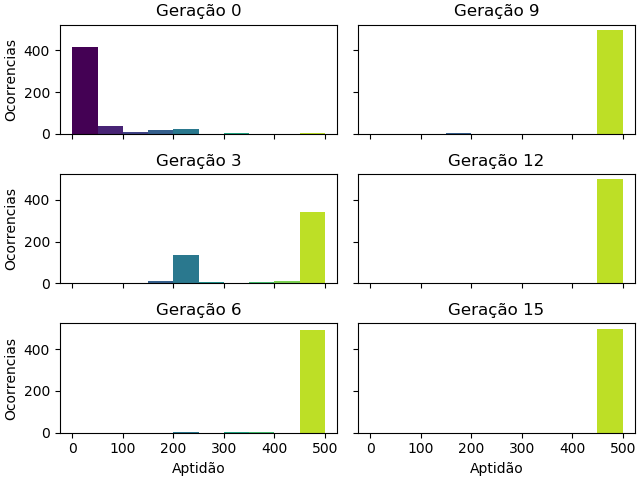
\includegraphics[width=0.8\textwidth]{02_desenvolvimento/04_EC_Fig_CartpoleAptHist.png}
	\caption{Número de indivíduos, em algumas gerações, que obtiveram cada faixa de aptidão.}
	\label{fig:4ec-cartpoleapthist}
\end{figure}

Conforme visto no Capítulo \ref{ssec:3deap-opgeneticos}, existe uma tendência de aumento do comprimento dos indivíduos ao longo do processo. O gráfico da Figura \ref{fig:4ec-cartpolecompr} mostra a média do comprimento de cada indivíduo em cada geração, assim como os valores mínimos e máximos observados. Já que todas as estatísticas foram obtidas através do valor médio em 10 execuções do algoritmo, o gráfico contém valores fracionários.

\begin{figure}[H]
	\centering
	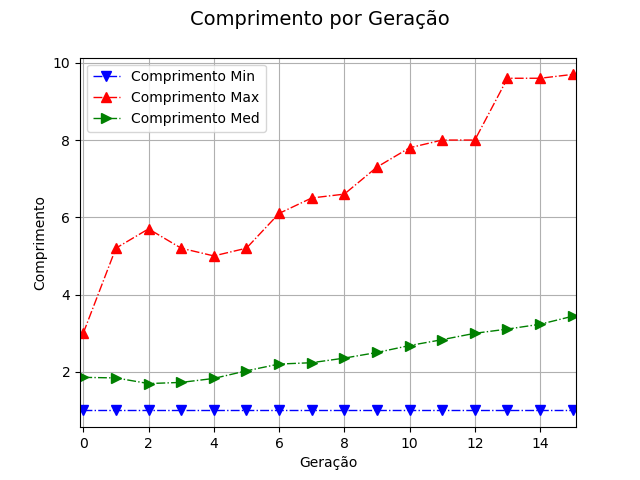
\includegraphics[width=0.8\textwidth]{02_desenvolvimento/04_EC_Fig_CartpoleCompr.png}
	\caption{Comprimento dos indivíduos por geração.}
	\label{fig:4ec-cartpolecompr}
\end{figure}

A complexidade dos indivíduos ao longo do processo pode ser observada no gráfico da Figura \ref{fig:4ec-cartpolecompl}.

\begin{figure}[H]
	\centering
	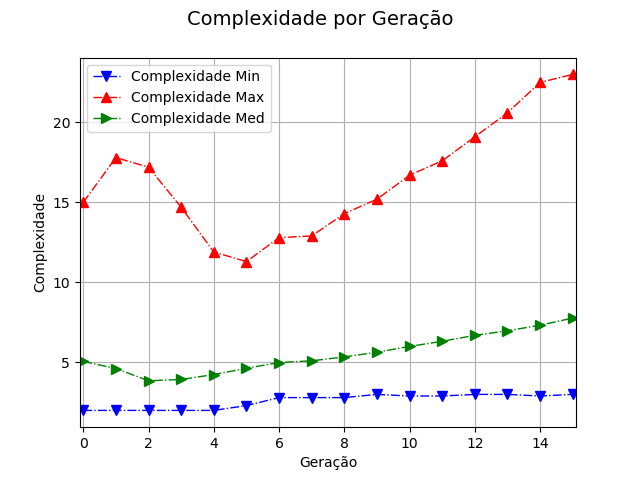
\includegraphics[width=0.8\textwidth]{02_desenvolvimento/04_EC_Fig_CartpoleCompl.png}
	\caption{Complexidade dos indivíduos em cada geração. }
	\label{fig:4ec-cartpolecompl}
\end{figure}

Foi possível observar que, alguns operadores e variáveis, pertencentes ao conjunto primitivo, são mais eficientes para a resolução do problema e tendem a aparecer com maior frequência à medida que a população se torna mais apta. Foi realizada a contagem dos operadores e variáveis de cada indivíduo pertencente à geração final, o resultado pode ser verificado no gráfico da Figura \ref{fig:4ec-cartpoleoper}.

\begin{figure}[H]
	\centering
	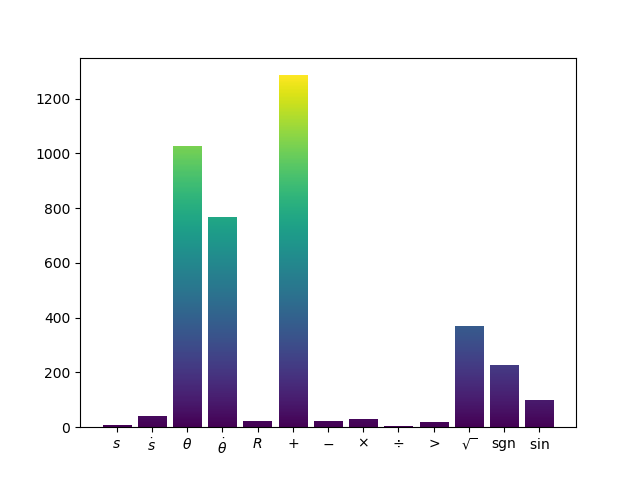
\includegraphics[width=0.8\textwidth]{02_desenvolvimento/04_EC_Fig_CartpoleOper.png}
	\caption{Número de ocorrências dos operadores e variáveis terminais, nos indivíduos da última geração.}
	\label{fig:4ec-cartpoleoper}
\end{figure}

Através do objeto \textit{hall da fama}, foi possível armazenar os indivíduos mais aptos que existiram na população ao longo de todo o processo de evolução. Esse objeto é atualizado a cada geração, de modo que o primeiro indivíduo possui a maior aptidão encontrada durante toda a execução do algoritmo evolucionário. Além disso, por ser um objeto de tamanho fixo, os indivíduos de gerações mais antigas possuem prioridade.

Na Figura \ref{fig:4ec-cartpoleindiv1}, é possível ver o primeiro indivíduo do hall da fama. Já que na geração inicial alguns indivíduos obtiveram a aptidão máxima, a solução da Figura \ref{fig:4ec-cartpoleindiv1} tem prioridade sobre as outras. O pequeno comprimento do indivíduo indica que, de fato, pertence às primeiras gerações.

\begin{figure}[H]
	\centering
	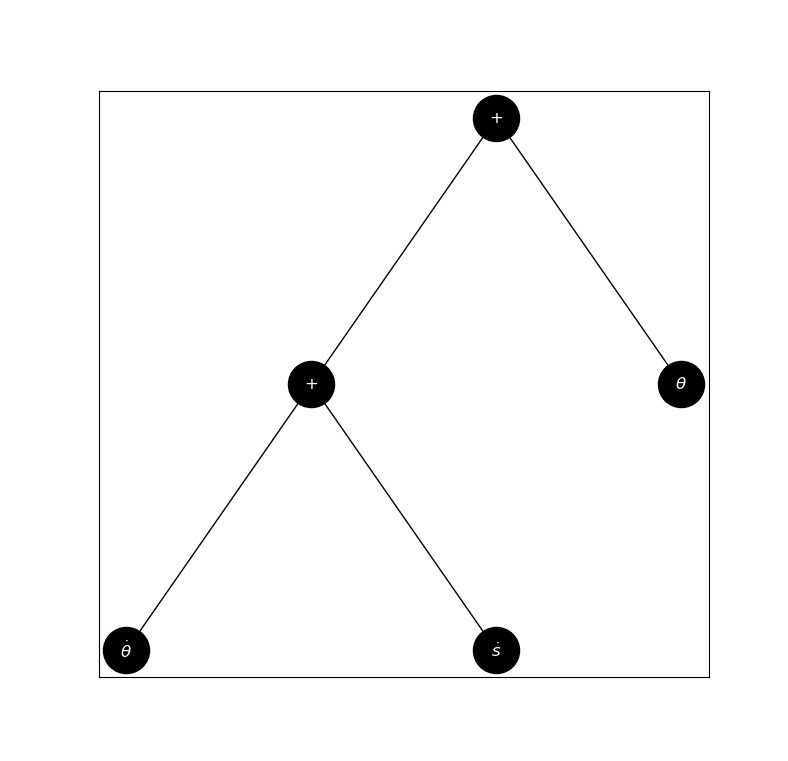
\includegraphics[width=\textwidth]{02_desenvolvimento/04_EC_Fig_CartpoleIndiv1.png}
	\caption{Primeiro indivíduo do hall da fama, na primeira execução do algoritmo.}
	\label{fig:4ec-cartpoleindiv1}
\end{figure}

É possível perceber indivíduos de maior comprimento, nas posições finais do hall da fama, como, por exemplo, na Figura \ref{fig:4ec-cartpoleindiv2}.

\begin{figure}[H]
	\centering
	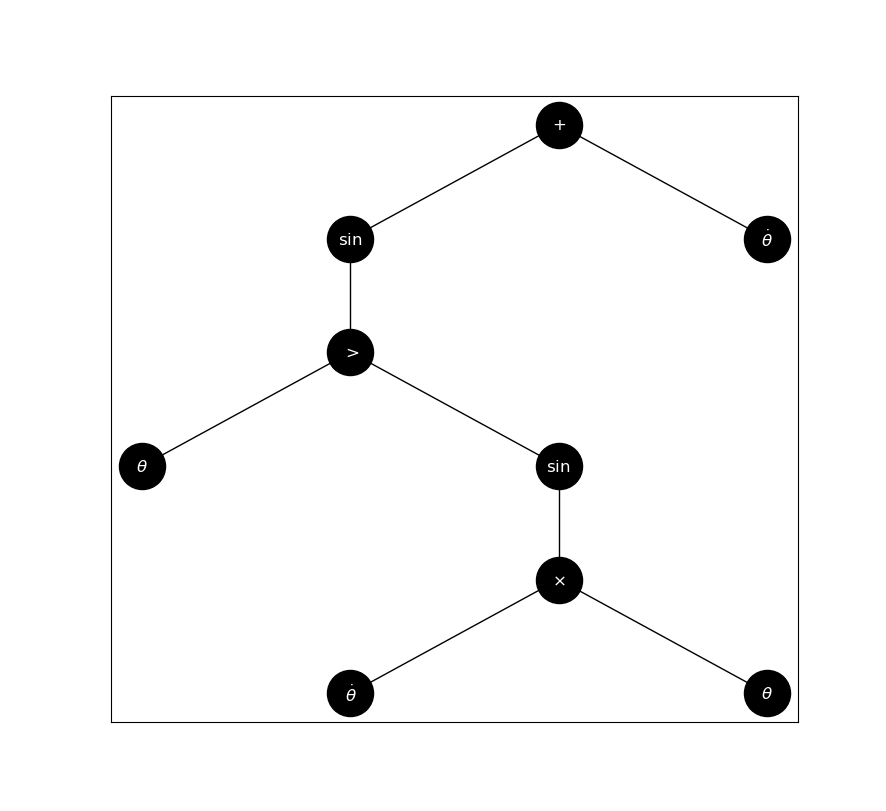
\includegraphics[width=\textwidth]{02_desenvolvimento/04_EC_Fig_CartpoleIndiv2.png}
	\caption{Vigésimo terceiro indivíduo do hall da fama, na primeira execução do algoritmo.}
	\label{fig:4ec-cartpoleindiv2}
\end{figure}

Já que múltiplos indivíduos obtiveram um bom desempenho em cada geração, incluindo as iniciais, é interessante notar o comprimento desses indivíduos mais aptos, especificamente. Pode-se observar que a tendência de aumento do comprimento dos indivíduos ao longo das gerações é preservada.

\begin{figure}[H]
	\centering
	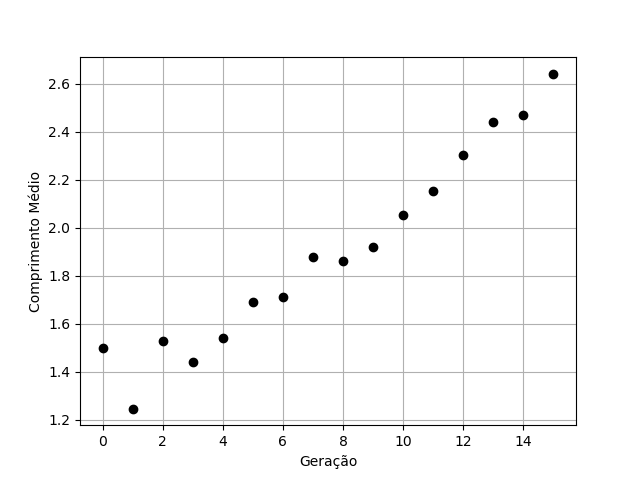
\includegraphics[width=0.7\textwidth]{02_desenvolvimento/compr_medio.png}
	\caption{Comprimento médio dos indivíduos que obtiveram aptidão maior que 400.}
	\label{fig:4ec-cartpolegrafaval}
\end{figure}

A Figura \ref{fig:4ec-cartpolegrafaval} mostra os gráficos relacionados à atuação do indivíduo da Figura \ref{fig:4ec-cartpoleindiv1}, em um único episódio. O eixo \textit{ação} indica o controle aplicado no sistema, a partir do \textit{resultado} obtido no cálculo da expressão matemática que representa um indivíduo.

\begin{figure}[H]
	\centering
	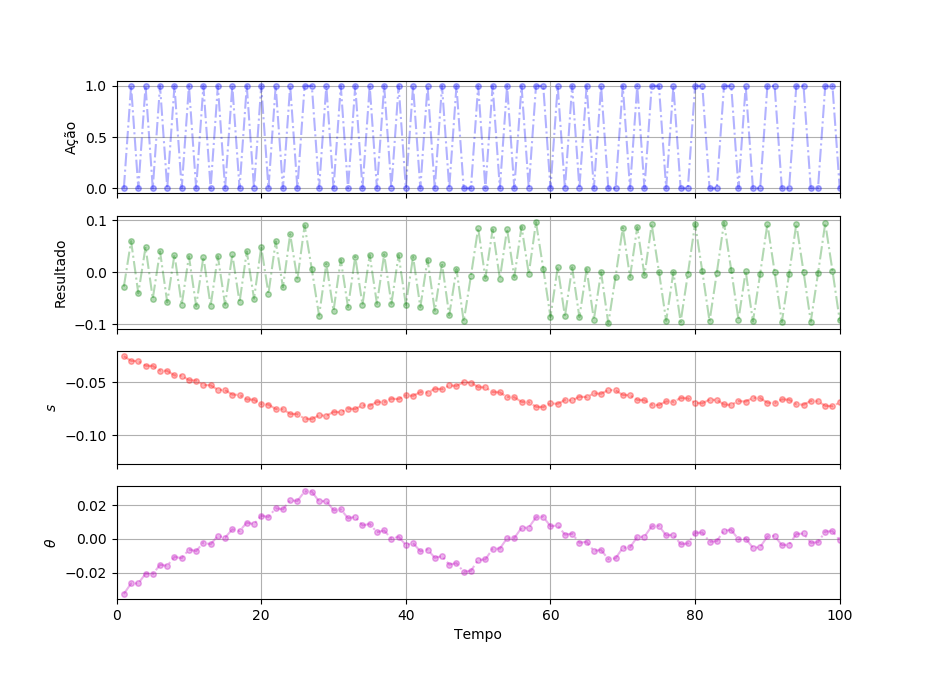
\includegraphics[width=\textwidth]{02_desenvolvimento/04_EC_Fig_CartpoleGraficosAval.png}
	\caption{Controle do sistema pelo indivíduo da Figura \ref{fig:4ec-cartpoleindiv1}. O pêndulo é levado rapidamente a um estado de baixa oscilação.}
	\label{fig:4ec-cartpolegrafaval}
\end{figure}

Foi possível observar que os indivíduos aptos pertencentes ao hall da fama são capazes de manter um valor baixo de oscilação do ângulo, ao redor do zero, entretanto, algumas soluções causavam a posição do carrinho a tender para um dos extremos, o que levava ao término antecipado do episódio.

Já que as aptidões dos indivíduos foram estimadas a partir de 10 simulações, é possível que as melhores soluções tenham sido beneficiadas por condições iniciais vantajosas. Não é possível, entretanto, aumentar o número de simulações sem que haja um aumento considerável no tempo de execução do algoritmo.

Dessa forma, é interessante verificar a aptidão dos indivíduos do hall da fama, em um grande número de episódios. Portanto, busca-se o indivíduo mais apto ao avaliar cada membro do hall da fama em 100 simulações.

A situação inicial do ambiente é determinada de forma aleatória, dentro de uma faixa específica característica de cada problema na biblioteca Gym. As condições iniciais de cada ambiente podem ser observadas no apêndice \ref{apendice:cond-iniciais}.

É proveitoso realizar a comparação desses resultados com a abordagem proposta pelo algoritmo DQN, uma vez que o critério de desempenho é o mesmo, isto é, a média de recompensa acumulada em vários episódios. O tempo médio de execução do algoritmo de PG foi \SI{334}{s}. O agente DQN é treinado, aproximadamente, pelo mesmo tempo. Em seguida, as recompensas médias acumuladas por episódio, em 100 simulações são comparadas. Destaca-se que a avaliação da PG foi realizada pelo indivíduo mais apto do hall da fama, quando cada membro é submetido à 100 episódios.

Utilizando a biblioteca \textit{stable-baselines} \cite{stable-baselines}, o agente DQN foi treinado por \SI{334}{s} (código encontra-se no apêndice). O gráfico da Figura \ref{fig:4ec-cartpoledqndiverg} mostra a recompensa obtida pelo agente ao longo do treinamento.

\begin{figure}[H]
	\centering
	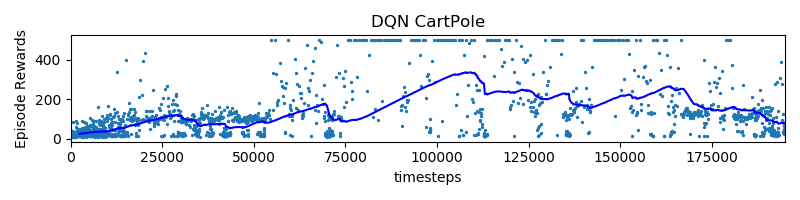
\includegraphics[width=0.85\textwidth]{02_desenvolvimento/04_EC_Fig_CartpoleDQNDiverg.png}
	\caption{Recompensa média acumulada em função do número de passos de simulação. A linha contínua representa a média móvel.}
	\label{fig:4ec-cartpoledqndiverg}
\end{figure}

Na Figura \ref{fig:4ec-cartpoledqndiverg} é possível notar a degradação da recompensa média acumulada a partir dos 110000 passos de simulação. Já que esse comportamento foi observado, o algoritmo foi executado novamente com o número de passos totais reduzido. O resultado pode ser verificado na Figura \ref{fig:4ec-cartpoledqngraf}.

\begin{figure}[H]
	\centering
	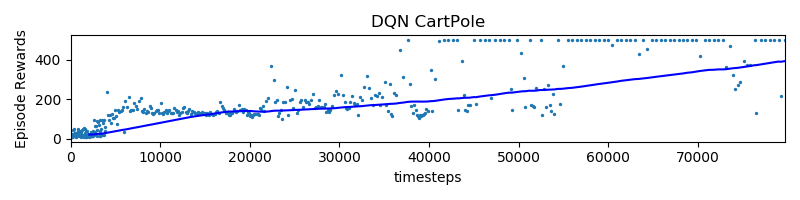
\includegraphics[width=0.85\textwidth]{02_desenvolvimento/04_EC_Fig_CartpoleDQNGraf.png}
	\caption{Recompensa média ao longo dos passos de simulação. A linha azul contínua indica a média móvel.}
	\label{fig:4ec-cartpoledqngraf}
\end{figure}

A Tabela \ref{tab:4ec-cartpolecomp} sumariza uma breve comparação entre o desempenho da programação genética com o algoritmo DQN, em termos de custos computacionais.

\begin{table}[H]
	\centering
	\begin{tabular}{SSS} \toprule
		{} & {{PG}} & {{DQN}} \\ \midrule
		{{Desempenho}} & {497} & {500} \\
		{{Tempo de execução (s)}} & {334} & {280} \\
		{{Passos de simulação}} & {16647338} & {80000} \\
		{{Número de episódios}} & {65095} & {450\footnotemark} \\
		\bottomrule
	\end{tabular}
	\caption{Comparação entre a programação genética e DQN, para o problema do pêndulo invertido.}\label{tab:4ec-cartpolecomp}
\end{table}

\footnotetext[1]{Valor estimado.}

A Figura \ref{fig:4ec-cartpoledqnvargraf} mostra a atuação do agente DQN, ao longo de um episódio.

\begin{figure}[H]
	\centering
	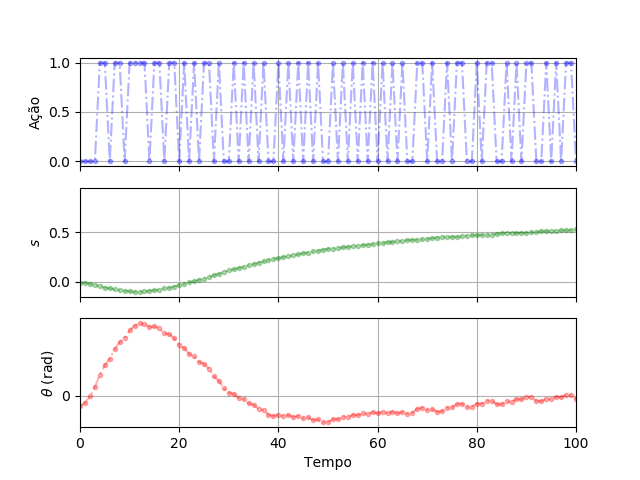
\includegraphics[width=0.85\textwidth]{02_desenvolvimento/04_EC_Fig_CartpoleDQNVarGraf.png}
	\caption{Posição do carrinho e ângulo do bastão, em função do tempo, com a atuação do agente DQN.}
	\label{fig:4ec-cartpoledqnvargraf}
\end{figure}

Observa-se, por fim, que as duas abordagens foram capazes de encontrar soluções satisfatórias para o problema. A seguir, serão abordados outros problemas que envolvem pêndulos e sua estabilização.

\subsection{Pêndulo \textit{Swing-up}}\label{ssec:4ec-pendulum}

O próximo sistema abordado está disponível na biblioteca Gym, na seção \textit{classic control}, direcionada à implementação de ambientes de simulações para problemas clássicos de controle. Conforme a abordagem do problema anterior, são introduzidos os critérios de término do episódio, as variáveis de estado observáveis e a implementação da recompensa. A formulação da função de aptidão, a partir da recompensa disponível, também é abordada.

A dinâmica envolve um bastão com uma de suas extremidades fixas, sendo possível a atuação do agente a partir da aplicação de um torque, em qualquer sentido, buscando a manutenção da extremidade livre na posição mais alta. A Figura \ref{fig:4ec-pendulumenv} ilustra o problema.

\begin{figure}[H]
	\centering
	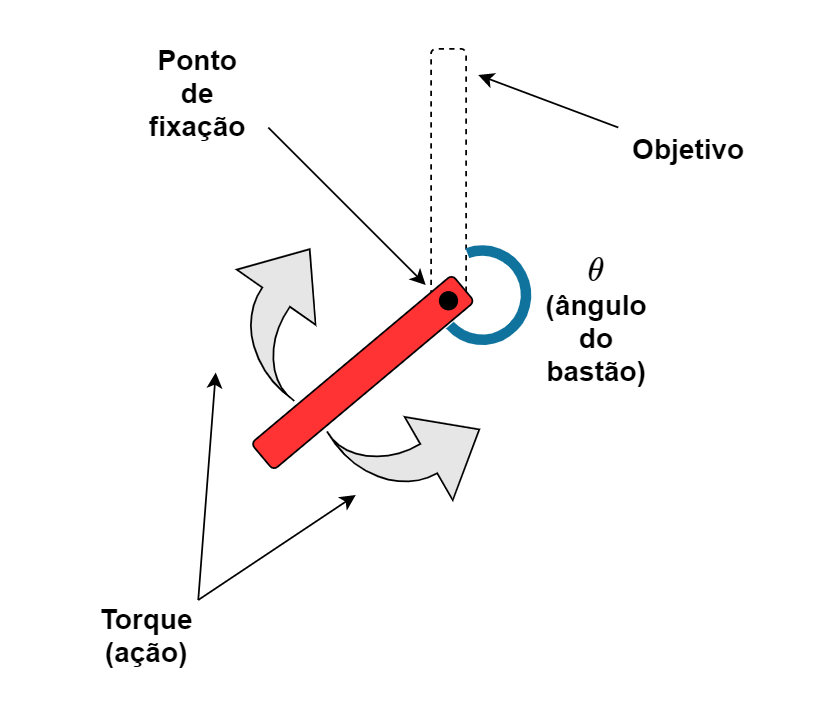
\includegraphics[width=0.7\textwidth]{02_desenvolvimento/04_EC_Fig_PendulumEnv2.png}
	\caption{Pêndulo \textit{Swing-up}.}
	\label{fig:4ec-pendulumenv}
\end{figure}

A seguir são enumerados alguns aspectos que aumentam a complexidade do problema, além de outras diferenças fundamentais do ambiente, em comparação com o pêndulo invertido:

\begin{itemize}[label=\raisebox{0.25ex}{\tiny$\bullet$}]
	\item O ponto de equilíbrio é estável.
	\item O torque aplicado em um único sentido, a partir da posição de repouso, não permite alcançar o objetivo em um movimento contínuo (o bastão precisa adquirir momento para superar a força gravitacional).
	\item As ações possíveis se dão no espaço contínuo.
	\item As recompensas são implementadas a partir de uma função custo.
\end{itemize}

A Tabela \ref{tab:4ec-pendulumvarestado} apresenta as variáveis que indicam o estado do sistema e que são fornecidas como uma \textit{observação}, após cada ação do agente. Já que o ponto de equilíbrio do sistema é estável, o único critério de término é o tempo de simulação. Com base na documentação da biblioteca Gym \cite{openaigym}, isto ocorre após 200 passos de simulação.

\begin{table}[H]
	\centering
	\caption{Variáveis que compõem a observação do pêndulo swing-up.}
	\label{tab:4ec-pendulumvarestado}
	\begin{tabular}{l|l} \toprule
		{Variável} & {Significado}\\ \midrule
		{$\cos(\theta)$} & {Cosseno do ângulo do bastão} \\
		{$\sin(\theta)$} & {Seno do ângulo do bastão} \\
		{$\dot{\theta}$} & {Velocidade angular do bastão} \\
		\bottomrule
	\end{tabular}
\end{table}

Seguindo a abordagem do Capítulo \ref{ssec:3deap-avalind}, é criada uma função de aptidão para o indivíduo. A recompensa a cada instante de tempo é uma função custo, segundo a Equação \ref{eq:4ec-pendulumrewardfunction}.

\begin{align}\label{eq:4ec-pendulumrewardfunction}
\begin{split}
r(t) = - \left[(\theta(t))^2 + 0,1(\dot\theta(t))^2+0,001(a(t))^2\right]\qquad &-\pi \le \theta \le \pi\\\\
&-2 \le a(t) \le 2
\end{split}
\end{align}

A variável $a(t)$ representa a ação (torque) do agente, no instante de tempo $t$. Foi mencionado no Capítulo \ref{sec:1pg-apg} a possibilidade de projetar a função de aptidão utilizando uma penalização por desvios de um estado de referência. Desta forma, o desempenho de um indivíduo é dado pela soma dos custos (implementados como recompensas negativas) em vários episódios:

\begin{align}\label{eq:4ec-pendulumaptidao}
\begin{split}
A(t) &= r(t) = - \left[\left[\theta(t)\right]^2 + 0,1\left[\dot\theta(t)\right]^2+0,001\left[a(t)\right]^2\right]\\\\
A_{tot}^{ep} &= \sum_{t=0}^{T} A(t) = - \sum_{t=0}^{T} \left[
\left[\theta(t)\right]^2 + 0,1\left[\dot\theta(t)\right]^2+0,001\left[a(t)\right]^2
\right]\qquad T \le 200\\\\
\bar{A} &= \dfrac{1}{nep}\sum_{ep=1}^{nep} A_{tot}^{ep} =
-\dfrac{1}{nep}\sum_{ep=1}^{nep}\sum_{t=0}^{T} \left[
\left[\theta(t)\right]^2 + 0,1\left[\dot\theta(t)\right]^2+0,001\left[a(t)\right]^2
\right]
\end{split}
\end{align}

De forma maneira similar ao problema anterior, o objetivo é \underline{maximizar} a aptidão média na Equação \ref{eq:4ec-pendulumaptidao}.

Buscando demonstrar a robustez da PG, poucas mudanças foram realizadas nos parâmetros da Tabela \ref{tab:4ec-param-cartpole}, mais especificamente, foram alterados: o número de entradas, comprimentos de inicialização e o comprimento máximo de mutação.

\begin{table}[H]
	\centering
	\begin{tabular}{l|l} \toprule
		{Parâmetro} & {Valor} \\ \midrule
		{Tamanho da População} & {500} \\
		{Probabilidade de Cruzamento} & {0,75} \\
		{Probabilidade de Mutação} & {0,05} \\
		{Número de Gerações} & {15} \\
		{Número de Entradas} & {3} \\
		{Faixa para Constante Efêmera} & {(-1, 1)} \\
		{Número de Simulações} & {10} \\
		{Tamanho do Campeonato de Aptidão} & {6} \\
		{Tamanho do Campeonato de Comprimento} & {1,2} \\
		{Operações} & {$+,\,-,\,\times,\,\div,\,\sqrt{},\,\sin,\,>$, sgn} \\
		{Comprimento Mínimo e Máximo de Inicialização} & {(2, 5)} \\
		{Comprimento Máximo de Mutação} & {7} \\
		{Limite de Comprimento dos Indivíduos} & {17} \\
		\bottomrule
	\end{tabular}
	\caption{Parâmetros da programação genética aplicada ao pêndulo swing-up.}\label{tab:4ec-pendulumparam}
\end{table}

É interessante destacar que o problema do Capítulo \ref{ssec:4ec-cartpole} utilizava ações discretas. Logo, bastava mapear os valores que resultavam da compilação das árvores em ações: números positivos produziam uma força para a direita no carrinho, enquanto os negativos geravam uma ação no sentido contrário.

Neste problema, o espaço de ações é contínuo, portanto é necessário apenas garantir que o resultado matemático da compilação de um indivíduo obedeça aos limites de torque, definidos na Equação \ref{eq:4ec-pendulumrewardfunction}. Isto pode ser concebido pela utilização da função \textit{clip}, cujo comportamento é demonstrado na Figura \ref{fig:4ec-pendulumclip}.

\begin{figure}[H]
	\centering
	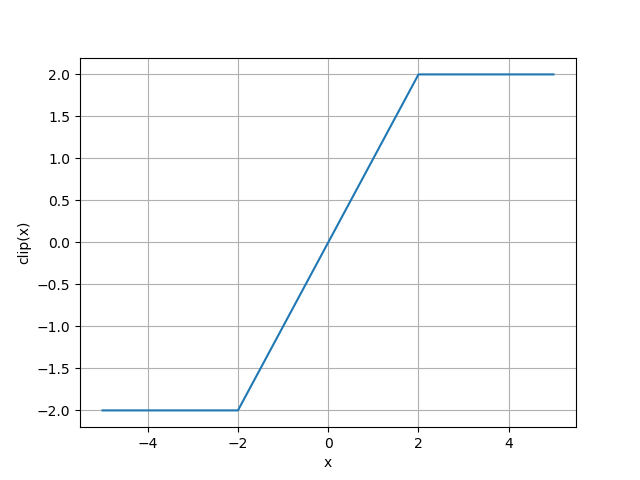
\includegraphics[width=0.82\textwidth]{02_desenvolvimento/04_EC_Fig_PendulumClipFun.png}
	\caption{Função \textit{clip}.}
	\label{fig:4ec-pendulumclip}
\end{figure}

Essa função funcionará como \textit{wrapper}, isto é, um mapeamento de um valor numérico em uma ação admissível.

Novamente, o algoritmo foi executado 10 vezes e a média das estatísticas foram obtidas. A começar pela aptidão ao longo das gerações, onde é possível perceber que a busca inicial da primeira geração, através da inicialização, não pôde obter um resultado satisfatório, como no problema anterior. As próximas gerações encontram uma solução eficaz para o pêndulo, conforme pode ser visto nas Figuras \ref{fig:4ec-pendulumaptger} e \ref{fig:4ec-pendulumapthist}.

\begin{figure}[H]
	\centering
	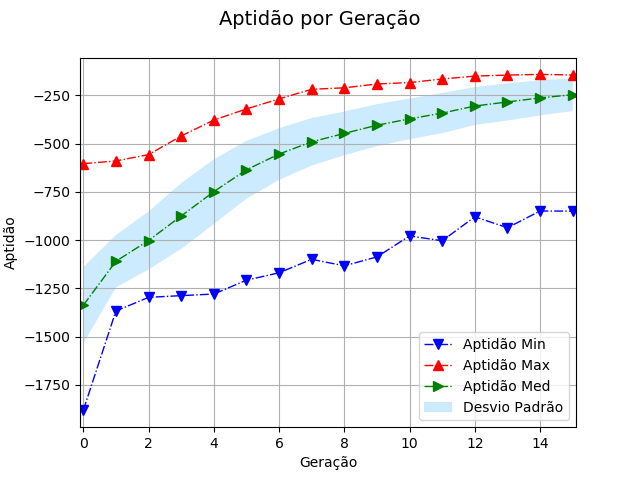
\includegraphics[width=0.85\textwidth]{02_desenvolvimento/04_EC_Fig_PendulumAptGer.png}
	\caption{Aptidão dos indivíduos, ao longo das gerações.}
	\label{fig:4ec-pendulumaptger}
\end{figure}

\begin{figure}[H]
	\centering
	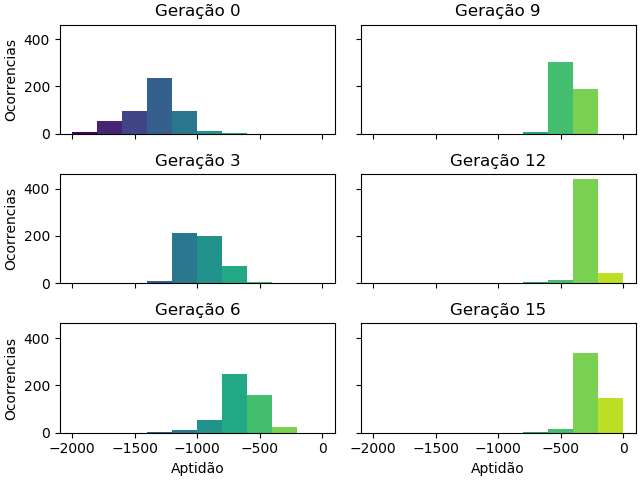
\includegraphics[width=0.85\textwidth]{02_desenvolvimento/04_EC_Fig_PendulumAptHist.png}
	\caption{Histograma da aptidão dos indivíduos.}
	\label{fig:4ec-pendulumapthist}
\end{figure}

O comprimento e a complexidade dos indivíduos da população, ao longo das gerações, podem ser vistos nas Figuras \ref{fig:4ec-pendulumcompr} e \ref{fig:4ec-pendulumcompl}, respectivamente.

\begin{figure}[H]
	\centering
	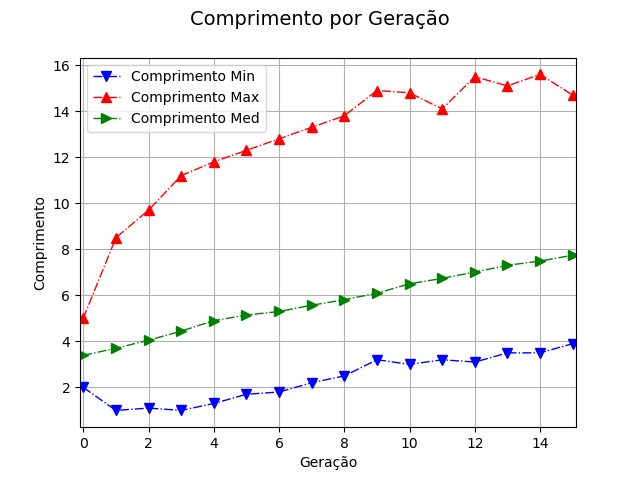
\includegraphics[width=0.85\textwidth]{02_desenvolvimento/04_EC_Fig_PendulumCompr.png}
	\caption{Comprimento dos indivíduos.}
	\label{fig:4ec-pendulumcompr}
\end{figure}

\begin{figure}[H]
	\centering
	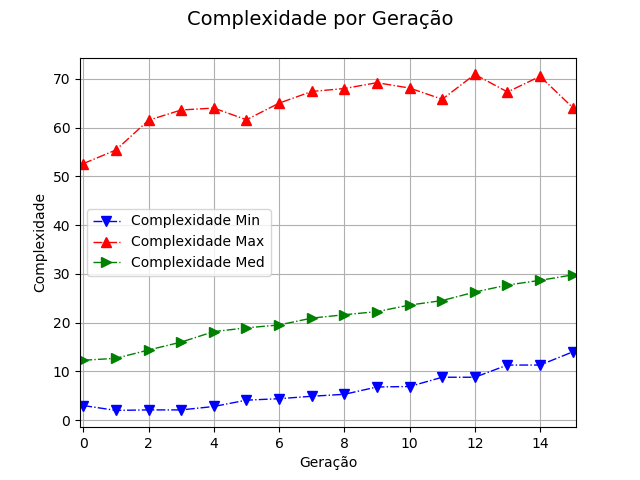
\includegraphics[width=0.85\textwidth]{02_desenvolvimento/04_EC_Fig_PendulumCompl.png}
	\caption{Complexidade dos indivíduos.}
	\label{fig:4ec-pendulumcompl}
\end{figure}

A Figura \ref{fig:4ec-pendulumoper} mostra o número de ocorrências dos operadores e variáveis terminais, na população da última geração.

\begin{figure}[H]
	\centering
	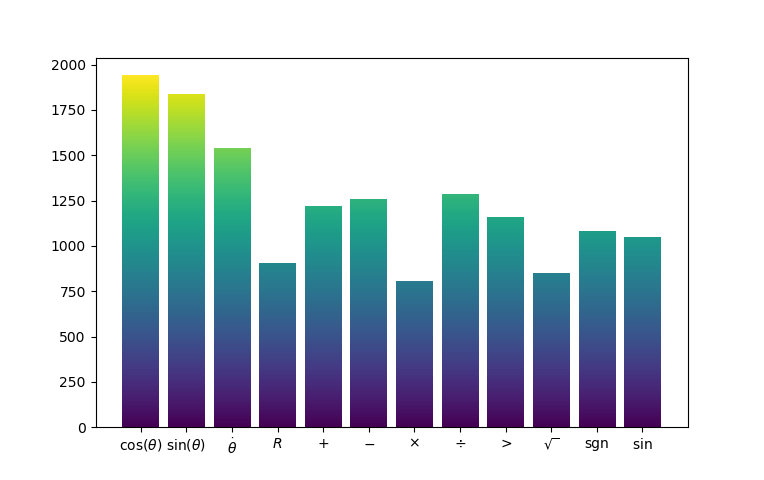
\includegraphics[width=0.85\textwidth]{02_desenvolvimento/04_EC_Fig_PendulumOper.png}
	\caption{Histograma de operadores e variáveis terminais, na última geração.}
	\label{fig:4ec-pendulumoper}
\end{figure}

O indivíduo de maior aptidão, na primeira execução, é mostrado na Figura \ref{fig:4ec-pendulumindiv1}.

\begin{figure}[H]
	\centering
	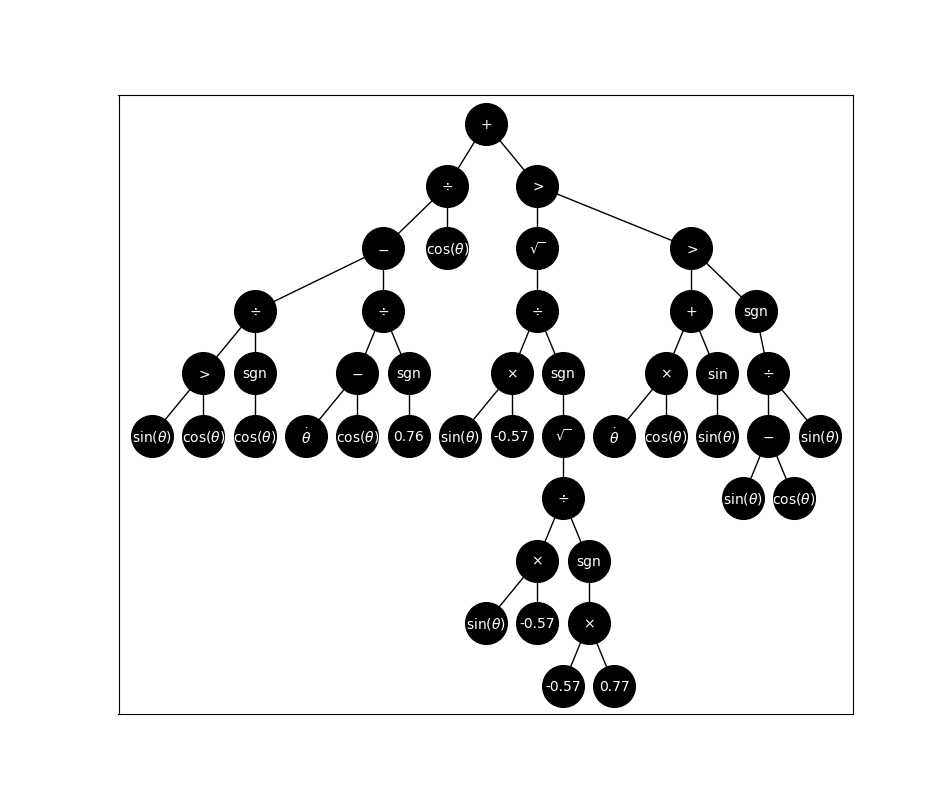
\includegraphics[width=\textwidth]{02_desenvolvimento/04_EC_Fig_PendulumIndiv1.png}
	\caption{Primeiro integrante do hall da fama.}
	\label{fig:4ec-pendulumindiv1}
\end{figure}

O segundo integrante do hall da fama, na primeira execução, é mostrado na Figura \ref{fig:4ec-pendulumindiv2}.

\begin{figure}[H]
	\centering
	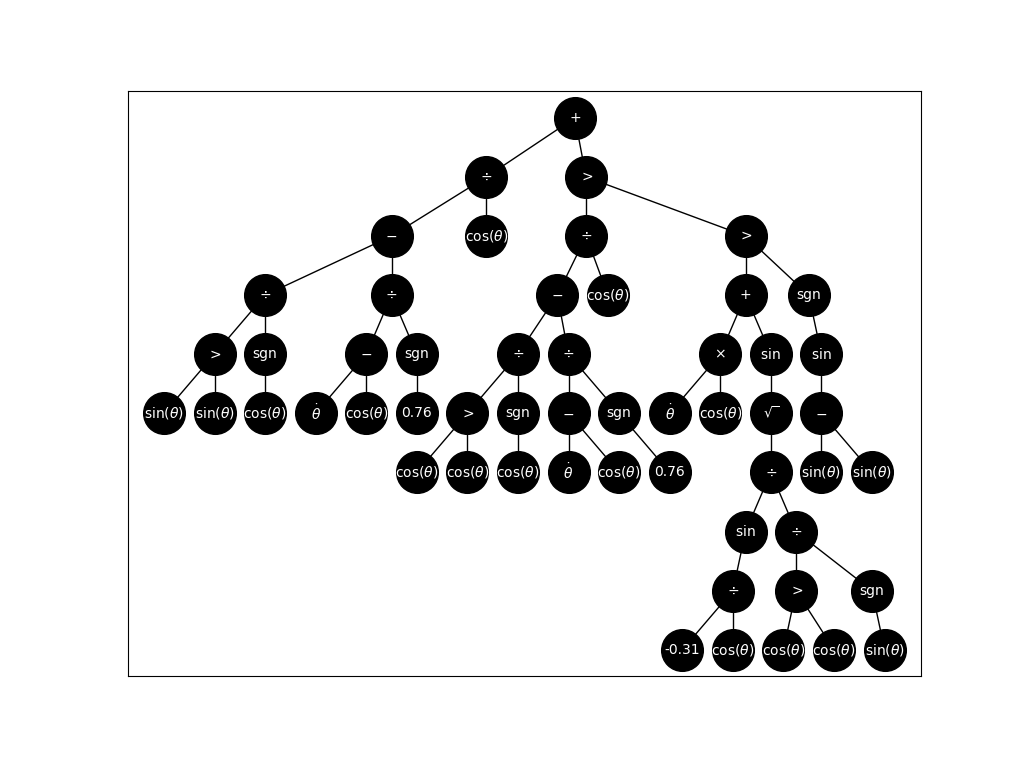
\includegraphics[width=\textwidth]{02_desenvolvimento/04_EC_Fig_PendulumIndiv2.png}
	\caption{Segundo integrante do hall da fama.}
	\label{fig:4ec-pendulumindiv2}
\end{figure}

A Figura \ref{fig:4ec-pendulumgraficosaval} mostra as ações, o ângulo e velocidade angular do bastão, quando o sistema é submetido ao controle do indivíduo da Figura \ref{fig:4ec-pendulumindiv1}, em um único episódio.

\begin{figure}[H]
	\centering
	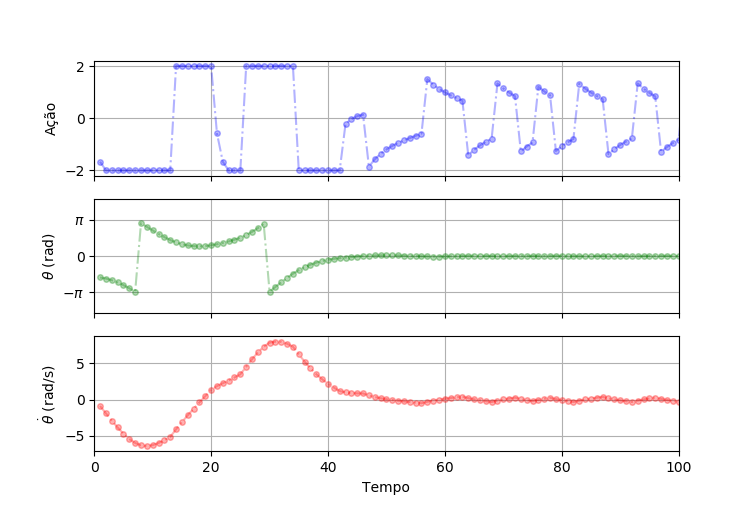
\includegraphics[width=0.95\textwidth]{02_desenvolvimento/04_EC_Fig_PendulumGraficosAval.png}
	\caption{Controle exercido pelo indivíduo da Figura \ref{fig:4ec-pendulumindiv1}.}
	\label{fig:4ec-pendulumgraficosaval}
\end{figure}

As transições bruscas no ângulo $\theta$ indicam a passagem da extremidade livre do pêndulo no ponto mais baixo, onde a função adquiri o maior valor absoluto. Após alguns instantes, o ângulo do bastão oscila em torno do zero de forma estável.

Utilizando a mesma metodologia do Capítulo \ref{ssec:4ec-cartpole}, é feita a avaliação em 100 episódios dos indivíduos do hall da fama. O maior valor de aptidão obtido é comparado com a recompensa acumulada de um agente treinado com o algoritmo DDPG, que pode ser visto como uma extensão do algoritmo DQN para ambientes com ações no espaço contínuo. Novamente, a medida de desempenho de um agente é obtida através função de recompensa disponibilizada pelo ambiente de simulação. Com isso, é possível realizar uma comparação direta entre as duas abordagens.

A Figura \ref{fig:4ec-pendulumddpggraf} mostra o agente DDPG sendo treinado em 100000 passos de tempo.

\begin{figure}[H]
	\centering
	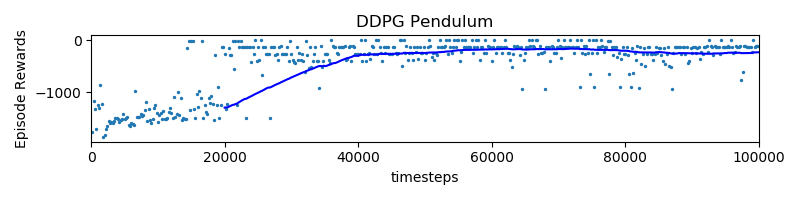
\includegraphics[width=0.9\textwidth]{02_desenvolvimento/04_EC_Fig_PendulumDDPGGraf.png}
	\caption{Evolução da recompensa acumulada para o agente DDPG no pêndulo swing-up.}
	\label{fig:4ec-pendulumddpggraf}
\end{figure}

A atuação do agente em um episódio pode ser vista na Figura \ref{fig:4ec-pendulumddpgvargraf}.

\begin{figure}[H]
	\centering
	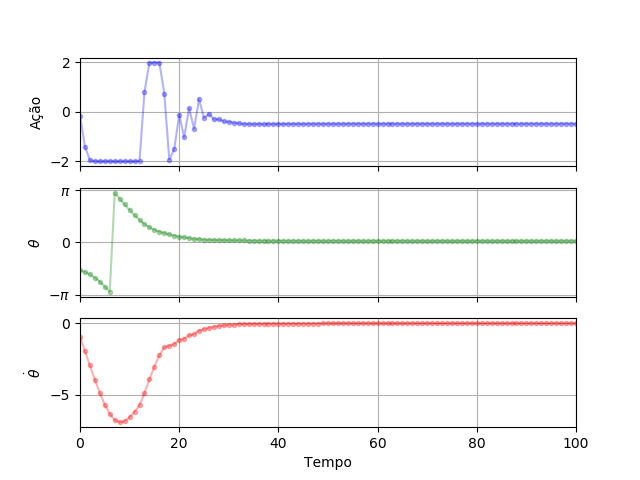
\includegraphics[width=0.9\textwidth]{02_desenvolvimento/04_EC_Fig_PendulumDDPGVarGraf.png}
	\caption{Dinâmica do pêndulo swing-up sob ação do agente DDPG.}
	\label{fig:4ec-pendulumddpgvargraf}
\end{figure}

\begin{table}[H]
	\centering
	\begin{tabular}{l|l|l} \toprule
		{} & {PG} & {{DDPG}} \\ \midrule
		{Desempenho} & {-230} & {-253} \\
		{Tempo de execução (s)} & {1649} & {194} \\
		{Passos de simulação} & {13034400} & {100000} \\
		{Número de episódios} & {65172} & {500} \\
		\bottomrule
	\end{tabular}
	\caption{Comparação entre a programação genética e DDPG para o pêndulo swing-up.}\label{tab:4ec-pendulumcomp}
\end{table}

É possível notar a partir da Tabela \ref{tab:4ec-pendulumcomp} que as duas abordagens são capazes de resolver o problema de controle proposto.

\subsection{Pêndulo Duplo Invertido}\label{ssec:4ec-dp}

Este problema é similar ao pêndulo invertido, pois a estabilização do bastão envolve a movimentação do veículo (que contém o ponto de fixação) sobre uma trilha. A diferença reside na existência de um outro bastão, fixado na extremidade antes livre, aumentando consideravelmente a complexidade do problema. As Figuras \ref{fig:4ec-dpenv} e \ref{fig:4ec-dpenv2} mostram o sistema proposto.

\begin{figure}[H]
	\centering
	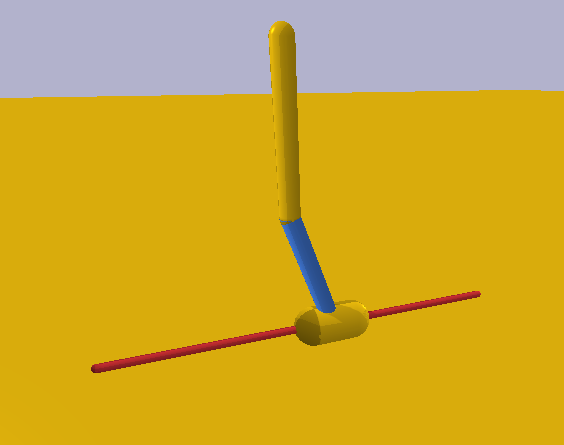
\includegraphics[width=0.8\textwidth]{02_desenvolvimento/04_EC_Fig_DPEnv.png}
	\caption{Renderização 3D do sistema pêndulo duplo invertido.}
	\label{fig:4ec-dpenv}
\end{figure}

\begin{figure}[H]
	\centering
	\includegraphics[width=0.8\textwidth]{02_desenvolvimento/04_EC_Fig_DPEnv2.png}
	\caption{Ângulos $\theta$, $\gamma$ e a posição do veículo ($s$).}
	\label{fig:4ec-dpenv2}
\end{figure}

A observação do sistema é composta de 11 variáveis:

\begin{table}[H]
	\centering
	\caption{Variáveis disponibilizadas como observação do pêndulo duplo invertido.}
	\label{tab:4ec-dpvarestado}
	\begin{tabular}{l|l} \toprule
		{Variável} & {Significado}\\ \midrule
		{$s$} & {Posição do carrinho} \\
		{$\sin(\theta)$} & {Seno do ângulo do bastão inferior} \\
		{$\sin{(\gamma)}$} & {Seno do ângulo do bastão superior} \\
		{$\cos(\theta)$} & {Cosseno do ângulo do bastão inferior} \\
		{$\cos(\gamma)$} & {Cosseno do ângulo do bastão superior} \\
		{$\dot{s}$} & {Velocidade do carrinho} \\
		{$\dot{\theta}$} & {Velocidade angular do bastão inferior} \\
		{$\dot{\gamma}$} & {Velocidade angular do bastão superior} \\
		{$f_r(s)$} & {Força de restrição em função da posição} \\
		{$f_r(\theta)$} & {Força de restrição em função de $\theta$} \\
		{$f_r(\gamma)$} & {Força de restrição em função de $\gamma$} \\
		\bottomrule
	\end{tabular}
\end{table}

Conforme a abordagem realizada até o momento, todas as variáveis da Tabela \ref{tab:4ec-dpvarestado} fazem parte do conjunto primitivo. Os outros parâmetros foram mantidos iguais ao do problema anterior (Tabela \ref{tab:4ec-pendulumparam}).

A função de recompensa do ambiente de simulação, a cada instante de tempo, pode ser vista na Equação \ref{eq:4ec-dprewardfunction}.

\begin{align}\label{eq:4ec-dprewardfunction}
\begin{split}
r(t) &= 10 - d_p(t) - v_p(t)\\\\
d_p(t) &= 0,01\left[s(t)\right]^2 + \left[y(t)-2\right]^2\\\\
v_p(t) &= 0,001\left[\dot{\theta}(t)\right]^2 + 0,005\left[\dot{\gamma}(t)\right]^2
\end{split}
\end{align}

Na Equação \ref{eq:4ec-dprewardfunction}, $d_p(t)$ e $v_p(t)$ são penalidades dadas em função da distância e das velocidades angulares dos bastões, respectivamente. A variável $y$ representa a altura da extremidade livre do bastão superior. Além de auxiliar no cálculo do custo, a quantidade $y$ também auxilia na verificação do término do episódio. Mais especificamente, a simulação encerra após 1000 passos de tempo ou quando a variável $y$ assume valores menores ou iguais a 1.

Naturalmente, a função de recompensa mostrada na Equação \ref{eq:4ec-dprewardfunction} será utilizada para o cálculo da aptidão de um indivíduo, utilizando a mesma formulação da Equação \ref{eq:4ec-pendulumaptidao}.

\begin{align}\label{eq:4ec-dpaptidao}
\begin{split}
A(t) &= r(t) = 10 - d_p(t) - v_p(t)\\\\
A_{tot}^{ep} &= \sum_{t=0}^{T} A(t) = - \sum_{t=0}^{T} \left[
10 - d_p(t) - v_p(t)
\right]\qquad T \le 1000\\\\
\bar{A} &= \dfrac{1}{nep}\sum_{ep=1}^{nep} A_{tot}^{ep} =
-\dfrac{1}{nep}\sum_{ep=1}^{nep}\sum_{t=0}^{T}
\left[
10 - d_p(t) - v_p(t)
\right]
\end{split}
\end{align}

Como o espaço de ações é contínuo, foi utilizada a função clip, da Figura \ref{fig:4ec-pendulumclip}, como wrapper para o resultado produzido pelas árvores. Entretanto, os valores extremos serão $-1$ e $1$, e não $-2$ e $2$.

As Figuras \ref{fig:4ec-dpapthist} a \ref{fig:4ec-dpcompl} mostram os resultados obtidos, através da média de 10 execuções do algoritmo.

\begin{figure}[H]
	\centering
	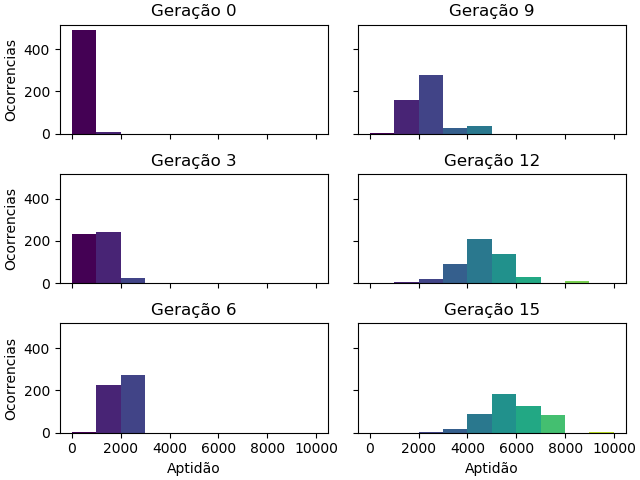
\includegraphics[width=0.8\textwidth]{02_desenvolvimento/04_EC_Fig_DPAptHist.png}
	\caption{Histograma da aptidão dos indivíduos, em algumas gerações, para o pêndulo duplo invertido.}
	\label{fig:4ec-dpapthist}
\end{figure}

\begin{figure}[H]
	\centering
	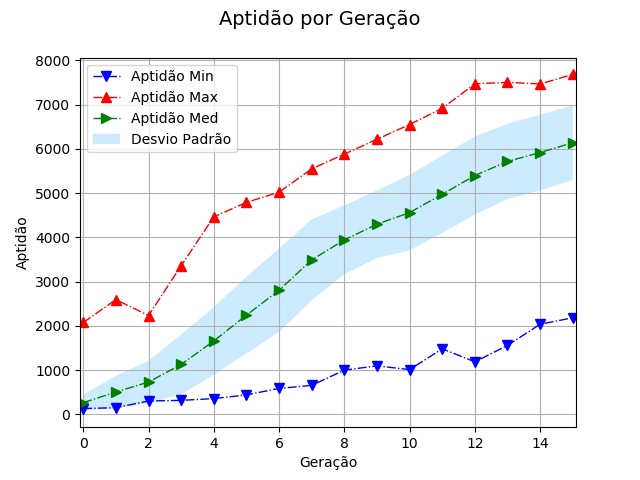
\includegraphics[width=0.8\textwidth]{02_desenvolvimento/04_EC_Fig_DPAptGer.png}
	\caption{Medidas de aptidão da população, em cada geração.}
	\label{fig:4ec-dpaptger}
\end{figure}

\begin{figure}[H]
	\centering
	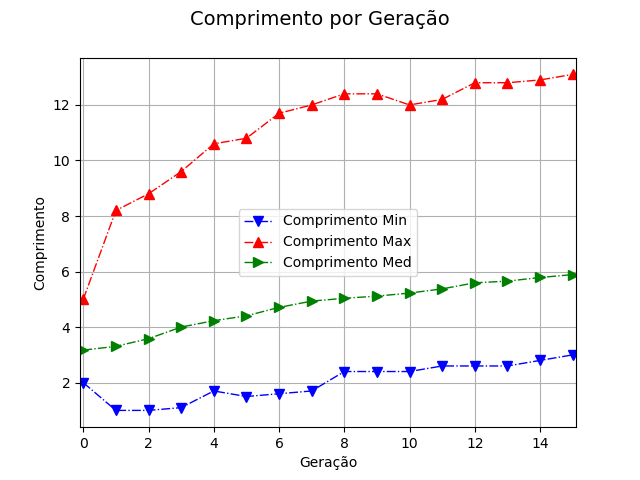
\includegraphics[width=0.8\textwidth]{02_desenvolvimento/04_EC_Fig_DPCompr.png}
	\caption{Medidas de comprimento da população, ao longo das gerações.}
	\label{fig:4ec-dpcompr}
\end{figure}

\begin{figure}[H]
	\centering
	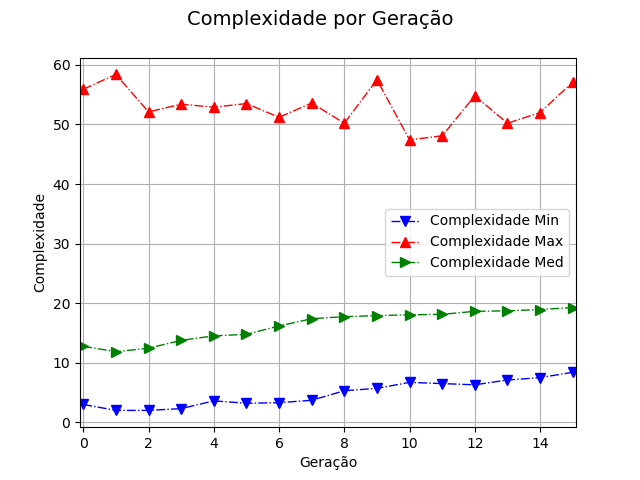
\includegraphics[width=0.8\textwidth]{02_desenvolvimento/04_EC_Fig_DPCompl.png}
	\caption{Medidas de complexidade dos indivíduos, em função das gerações.}
	\label{fig:4ec-dpcompl}
\end{figure}

\begin{figure}[H]
	\centering
	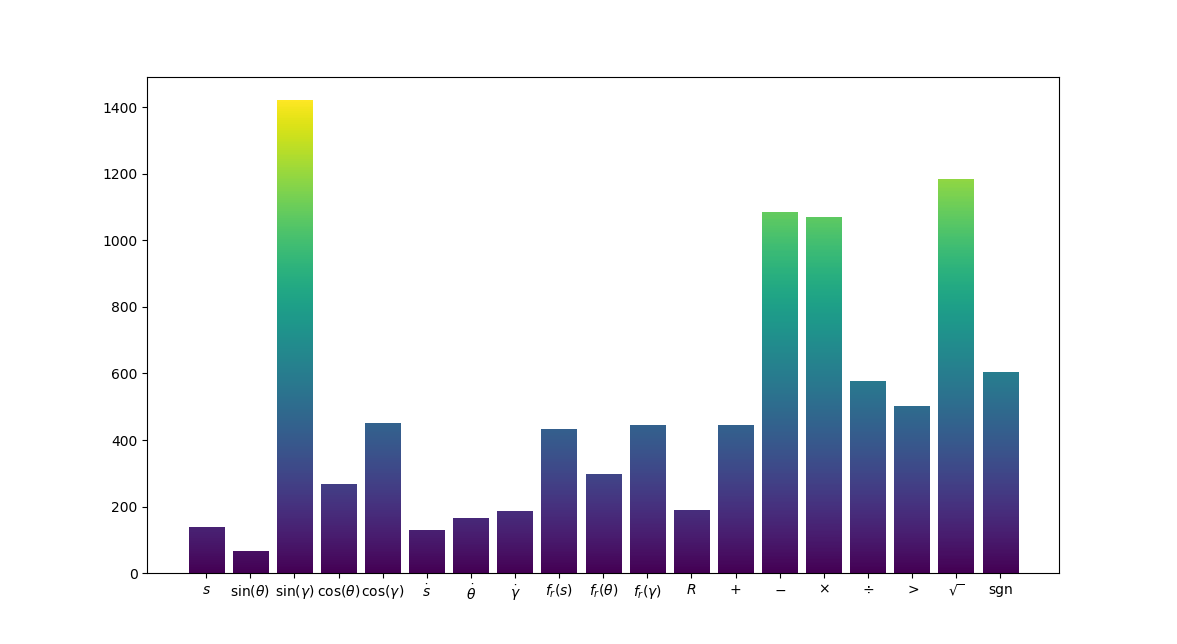
\includegraphics[width=\textwidth]{02_desenvolvimento/04_EC_Fig_DPOperHist.png}
	\caption{Número de ocorrências dos operadores e variáveis terminais, na última geração.}
	\label{fig:4ec-dpoperhist}
\end{figure}

Para cada indivíduo do hall da fama foram realizadas 100 simulações, com o intuito de verificar a solução mais apta e generalista. O indivíduo da Figura \ref{fig:4ec-dpindiv1} obteve uma aptidão média de 7794.

\begin{figure}[H]
	\centering
	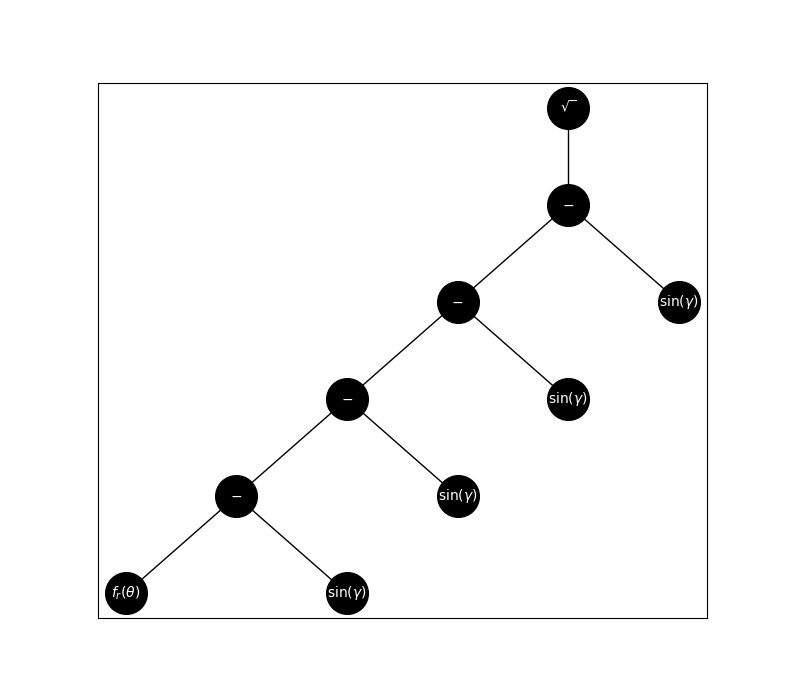
\includegraphics[width=0.9\textwidth]{02_desenvolvimento/04_EC_Fig_DPIndiv1}
	\caption{Indivíduo mais apto da primeira execução do algoritmo.}
	\label{fig:4ec-dpindiv1}
\end{figure}

Os gráficos da Figura \ref{fig:4ec-dpvargraf} mostram os ângulos e a posição do carrinho, quando a solução da Figura \ref{fig:4ec-dpindiv1} atua em um episódio.

\begin{figure}[H]
	\centering
	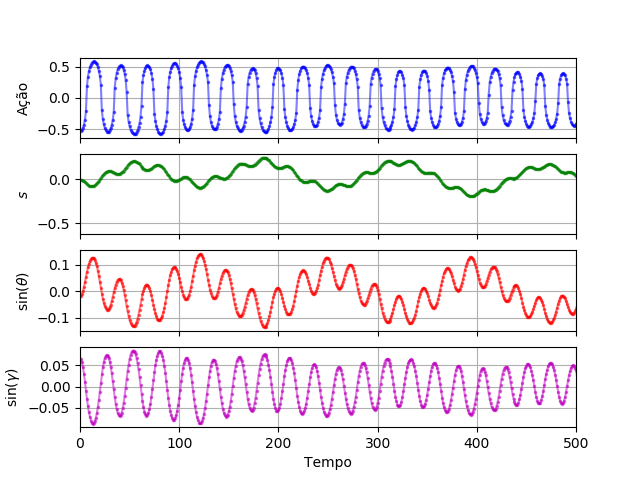
\includegraphics[width=0.9\textwidth]{02_desenvolvimento/04_EC_Fig_DPVarGraf}
	\caption{Avaliação do melhor indivíduo observado na primeira execução.}
	\label{fig:4ec-dpvargraf}
\end{figure}

O gráfico da Figura \ref{fig:4ec-dpddpgtrain} mostra um agente sendo treinado com o algoritmo DDPG, por 400000 passos de simulação. A recompensa média acumulada pelo agente, em 100 episódios, pode ser vista na Tabela \ref{tab:4ec-dpcomp}, junto à outras estatísticas relacionadas ao custo computacional.

\begin{figure}[H]
	\centering
	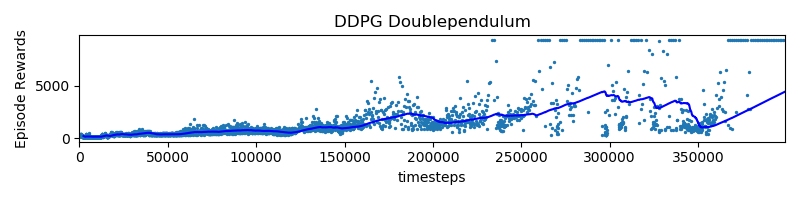
\includegraphics[width=\textwidth]{02_desenvolvimento/04_EC_Fig_DPDDPGTrain}
	\caption{Evolução da recompensa acumulada do agente DDPG. A linha azul representa a média móvel.}
	\label{fig:4ec-dpddpgtrain}
\end{figure}

\begin{table}[H]
	\centering
	\begin{tabular}{l|l|l} \toprule
		{} & {{PG}} & {{DDPG}} \\ \midrule
		{{Desempenho}} & {7794} & {9019} \\
		{{Tempo de execução (s)}} & {2406} & {1230} \\
		{{Passos de simulação}} & {10392643} & {400000} \\
		{{Número de episódios}} & {64989} & {1230} \\
		\bottomrule
	\end{tabular}
	\caption{Comparação entre PG e DDPG para o pêndulo duplo invertido.}\label{tab:4ec-dpcomp}
\end{table}

\subsection{Carro na Ladeira}\label{ssec:4ec-mc}

O problema do carro na ladeira foi descrito inicialmente por Andrew Moore \cite{moore1990efficient} e se tornou um dos problemas mais importantes na teoria de aprendizagem por reforço. O problema consiste em um carro cujo objetivo é chegar ao topo de uma montanha, com uma determinada velocidade. Entretanto, o motor não é forte o suficiente a ponto de permitir que o carro chegue no objetivo em um único movimento. É necessário, portanto, que o carro ganhe energia ao se locomover na direção contrária. A Figura \ref{fig:4ec-mcenv} ilustra o problema.

\begin{figure}[H]
	\centering
	\includegraphics[width=0.8\textwidth]{02_desenvolvimento/04_EC_Fig_MCEnv.png}
	\caption{Problema do carro na ladeira.}
	\label{fig:4ec-mcenv}
\end{figure}

A implementação do ambiente na biblioteca permite definir qual a velocidade que o carro precisa ter ao chegar no topo da montanha. A configuração padrão, que será utilizada, não impõe um valor mínimo de velocidade. Dessa forma, basta que o carro chegue à posição indicada pela bandeira, na Figura \ref{fig:4ec-mcenv}.

A observação do ambiente é simples, e consiste apenas na posição e velocidade do carro, conforme a Tabela \ref{tab:4ec-mcvarestado} indica. O agente recebe uma penalização unitária, conforme indica a Equação \ref{eq:4ec-mcrewardfunction}, a cada instante de tempo. Desta forma, a busca é por indivíduos que cheguem ao objetivo no menor tempo possível.

\begin{table}[H]
	\centering
	\caption{Variáveis de estado para o problema do carro na ladeira.}
	\label{tab:4ec-mcvarestado}
	\begin{tabular}{l|l} \toprule
		{Variável} & {Significado}\\ \midrule
		{$s$} & {Posição do carro.} \\
		{$\dot{s}$} & {Velocidade do carro} \\
		\bottomrule
	\end{tabular}
\end{table}

\begin{equation}\label{eq:4ec-mcrewardfunction}
r(t) = -1
\end{equation}

O espaço de ações é discreto e indica uma força que atua no veículo, de acordo com a Equação \ref{eq:4ec-mcactions}.

\begin{equation}\label{eq:4ec-mcactions}
a(t) =
\begin{cases}
0 \quad \longrightarrow \quad \text{Força aplicada à esquerda}\\
1 \quad \longrightarrow \quad \text{Não aplica força}\\
2 \quad \longrightarrow \quad \text{Força aplicada à direita}\\
\end{cases}
\end{equation}

No capítulo \ref{ssec:4ec-cartpole} foi visto como transformar um número no espaço contínuo, retornado pela função de controle de um indivíduo, em uma ação mapeada em números inteiros. Com um conjunto de duas ações possíveis, bastava mapear números positivos à uma ação e negativos à outra. No problema atual, existem três ações possíveis, portanto, é definida uma faixa de valores para a situação em que não se aplica força , isto é, quando $a(t)$ vale $1$. Este artifício pode ser conferido na Equação \ref{eq:4ec-mcwrapper}, onde $num(t)$ representa a saída da função de controle do indivíduo, no instante $t$.

\begin{equation}\label{eq:4ec-mcwrapper}
	a(t)=\begin{cases}
	0,\qquad\text{se $num(t) \le$ -0,5}\\
	1,\qquad\text{se -0,5 $< num(t) \le$ 0,5}\\
	2,\qquad\text{se 0,5 $< num(t)$}
	\end{cases}
\end{equation}

Utilizando a mesma abordagem dos problemas anteriores, a aptidão de um indivíduo será a média da recompensa acumulada, em um determinado número de episódios.

\begin{equation}\label{eq:4ec-mcaptidao}
\bar{A} =
\dfrac{1}{nep}\sum_{ep=1}^{nep}\sum_{t=0}^{T} r(t)
\end{equation}

A Tabela \ref{tab:4ec-mcparam} mostra os parâmetros utilizados na execução da PG.

\begin{table}[H]
	\centering
	\begin{tabular}{l|l} \toprule
		{Parâmetro} & {Valor} \\ \midrule
		{Tamanho da População} & {500} \\
		{Probabilidade de Cruzamento} & {0,70} \\
		{Probabilidade de Mutação} & {0,10} \\
		{Número de Gerações} & {15} \\
		{Número de Entradas} & {4} \\
		{Faixa para Constante Efêmera} & {(-1, 1)} \\
		{Número de Simulações} & {10} \\
		{Tamanho do Campeonato de Aptidão} & {6} \\
		{Tamanho do Campeonato de Comprimento} & {1,2} \\
		{Operações} & {$+,\,-,\,\times,\,\div,\,\sqrt{},\,\sin,\,>$, sgn} \\
		{Comprimento Mínimo e Máximo de Inicialização} & {(2, 5)} \\
		{Comprimento Máximo de Mutação} & {9} \\
		{Limite de Comprimento dos Indivíduos} & {17} \\
		\bottomrule
	\end{tabular}
	\caption{Parâmetros utilizados para o problema do carro na ladeira.}\label{tab:4ec-mcparam}
\end{table}

Os resultados obtidos são mostrados nas Figuras \ref{fig:4ec-mcapthist} a \ref{fig:4ec-mcoperhist}.

\begin{figure}[H]
	\centering
	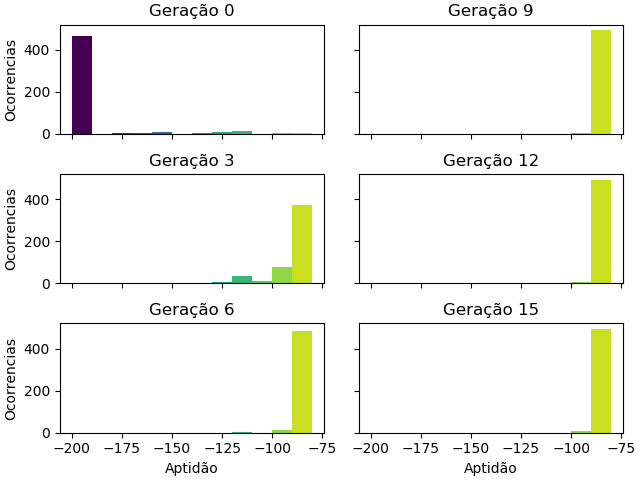
\includegraphics[width=0.8\textwidth]{02_desenvolvimento/04_EC_Fig_MCAptHist.png}
	\caption{Histograma da aptidão dos indivíduos, em algumas gerações, para o pêndulo duplo invertido.}
	\label{fig:4ec-mcapthist}
\end{figure}

\begin{figure}[H]
	\centering
	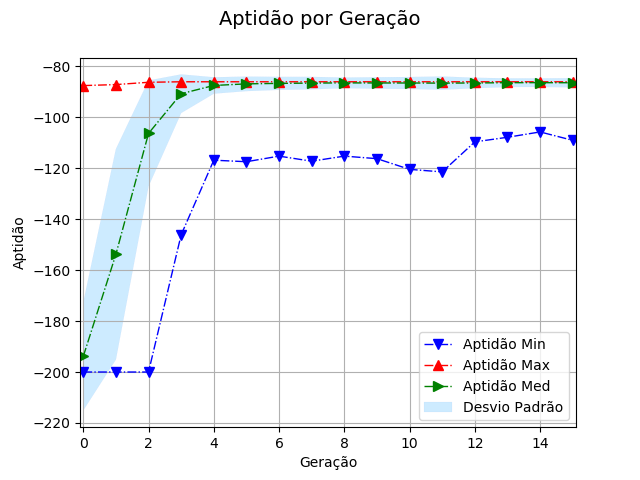
\includegraphics[width=0.8\textwidth]{02_desenvolvimento/04_EC_Fig_MCAptGer.png}
	\caption{Aptidão da população.}
	\label{fig:4ec-mcaptger}
\end{figure}

\begin{figure}[H]
	\centering
	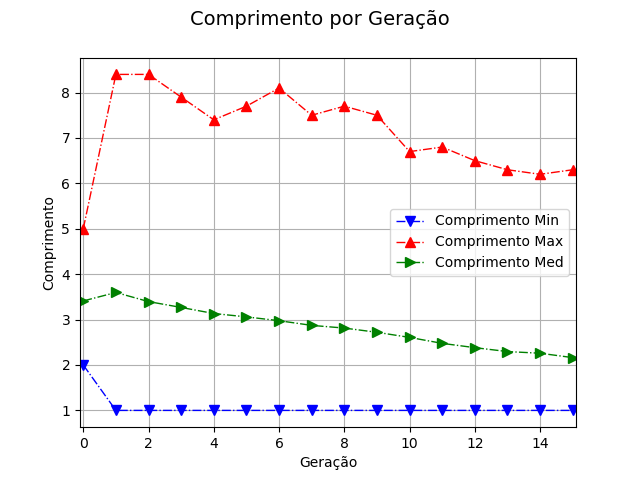
\includegraphics[width=0.8\textwidth]{02_desenvolvimento/04_EC_Fig_MCCompr.png}
	\caption{Comprimento dos indivíduos.}
	\label{fig:4ec-mccompr}
\end{figure}

\begin{figure}[H]
	\centering
	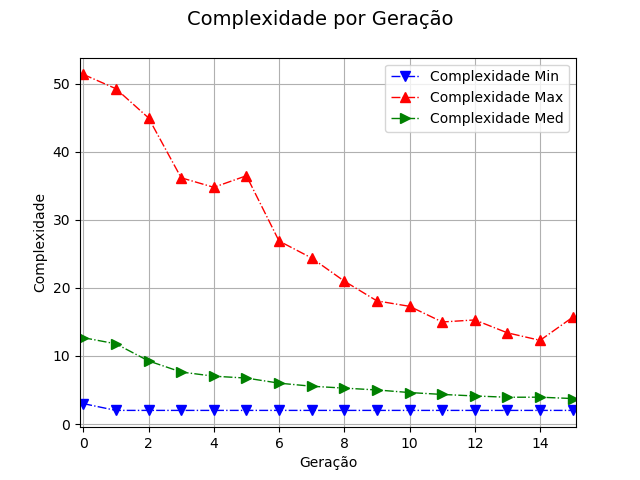
\includegraphics[width=0.8\textwidth]{02_desenvolvimento/04_EC_Fig_MCCompl.png}
	\caption{Complexidade da população.}
	\label{fig:4ec-mccompl}
\end{figure}

\begin{figure}[H]
	\centering
	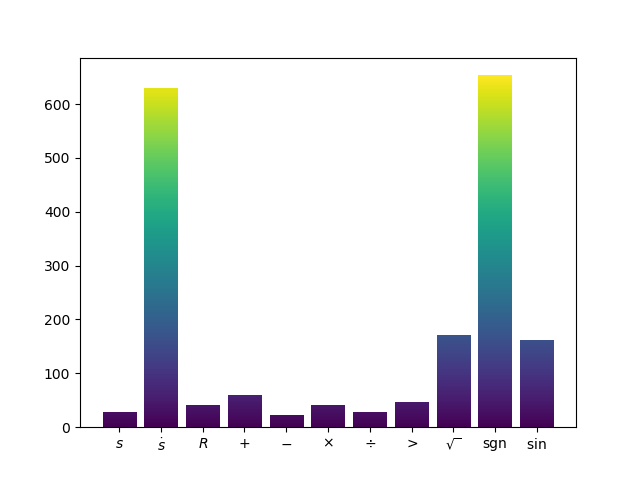
\includegraphics[width=0.8\textwidth]{02_desenvolvimento/04_EC_Fig_MCOperHist.png}
	\caption{Ocorrências dos operadores e variáveis terminais, na última geração.}
	\label{fig:4ec-mcoperhist}
\end{figure}

O melhor indivíduo foi obtido ao simular a atuação de todas as soluções do hall da fama, em 100 episódios. A Figura \ref{fig:4ec-mcindiv1} mostra a composição do indivíduo.

\begin{figure}[H]
	\centering
	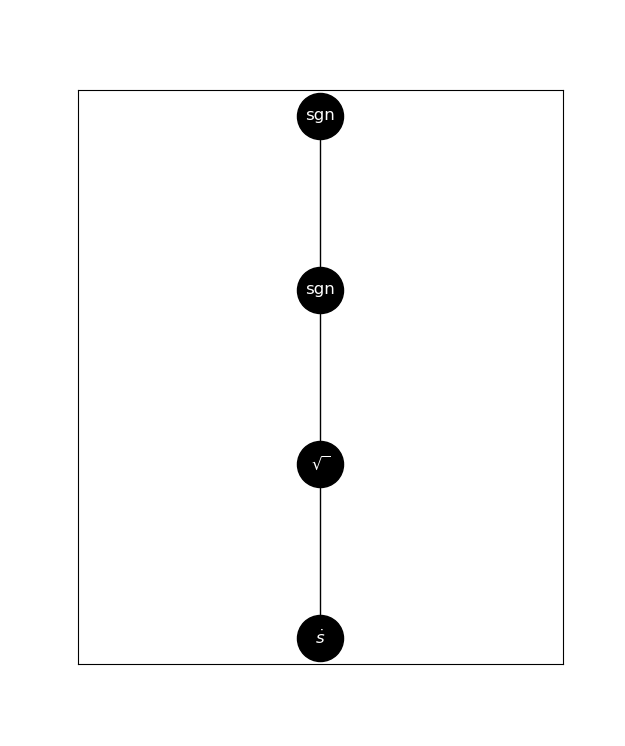
\includegraphics[width=0.8\textwidth]{02_desenvolvimento/04_EC_Fig_MCIndiv1.png}
	\caption{Melhor indivíduo da primeira execução.}
	\label{fig:4ec-mcindiv1}
\end{figure}

\begin{figure}[H]
	\centering
	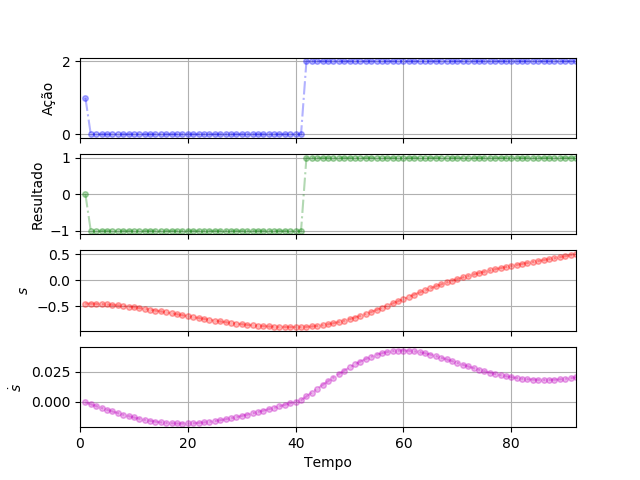
\includegraphics[width=0.8\textwidth]{02_desenvolvimento/04_EC_Fig_MCVarAval}
	\caption{Atuação do indivíduo da Figura \ref{fig:4ec-mcindiv1} em um episódio aleatório.}
	\label{fig:4ec-mcvaraval}
\end{figure}

Como o espaço de ações é discreto, um agente foi treinado utilizando o algoritmo DQN. A Figura \ref{fig:4ec-mcdqntrain} mostra a recompensa acumulada pelo agente DQN ao longo do tempo de execução. A Tabela \ref{tab:4ec-mccomp} sumariza os resultados encontrados com a PG, comparado à outra abordagem.

\begin{figure}[H]
	\centering
	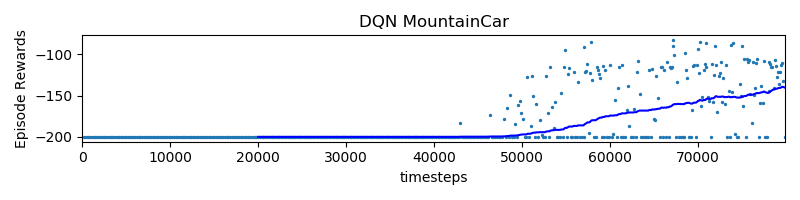
\includegraphics[width=0.9\textwidth]{02_desenvolvimento/04_EC_Fig_MCDQNTrain.png}
	\caption{Agente DQN e a recompensa acumulada ao longo dos passos de tempo.}
	\label{fig:4ec-mcdqntrain}
\end{figure}

\begin{table}[H]
	\centering
	\begin{tabular}{l|l|l} \toprule
		{} & {{PG}} & {{DQN}} \\ \midrule
		{{Desempenho}} & {-108} & {-140} \\
		{{Tempo de execução (s)}} & {79} & {311} \\
		{{Passos de simulação}} & {966211} & {80000} \\
		{{Número de episódios}} & {6514} & {450\footnotemark} \\
		\bottomrule
	\end{tabular}
	\caption{Comparação entre PG e DQN para o problema do carro na ladeira.}\label{tab:4ec-mccomp}
\end{table}

\footnotetext[2]{Valor aproximado.}

É possível perceber, em termos de tempo de execução, que a PG se mostrou bem superior ao algoritmo DQN.


\subsection{Veículo Terrestre Autônomo}\label{ssec:4ec-carrinho}

O último problema abordado trata do planejamento de trajetória para um veículo autônomo semelhante a um automóvel de passeio. O veículo é propelido através do torque aplicado às rodas dianteiras, as quais também dão direção ao movimento permitindo a mudança de orientação do veículo em trajetórias curvas.

A cinemática do veículo é dada pela Equação \ref{eq:4ec-carrinhosisteq}, nas quais a velocidade $v$ e a orientação $\phi$ das rodas dianteiras são os sinais de controle do movimento, enquanto $x$, $y$ e $\theta$ representam as coordenadas do centro de gravidade do veículo (origem do sistema de coordenadas fixo ao veículo) com relação a um sistema de coordenadas fixo de referência e a orientação entre ambos, respectivamente. L é a distância entre os eixos traseiro e dianteiro. 

\begin{align}\label{eq:4ec-carrinhosisteq}
\begin{split}
\dot{x_c}&=v\cos(\theta+\beta)\\
\dot{y_c}&=v\sin(\theta+\beta)\\
\dot{\theta}&=\dfrac{v\cos\beta\tan\phi}{L}\\
\beta&=\arctan\left(\dfrac{\tan\phi}{2}\right)
\end{split}
\end{align}

A Figura \ref{fig:4ec-carrinhofigsisteq} apresenta o modelo cinemático de ``bicicleta'' em que se baseia a Equação \ref{eq:4ec-carrinhosisteq}. Neste modelo, é realizada uma simplificação da cinemática de veículos de passeio, ao considerar que as rodas dos eixos frontrais e traseiros se unem no centro geométrico de cada eixo. Dessa forma, considera-se a existência de apenas duas rodas no veículo, equiparando-se a uma bicicleta, conforme indica a Figura \ref{fig:4ec-carrinhofigsisteq}. Apesar de sua simplicidade, o modelo se mostra eficiente para veículos com baixa aceleração \cite{bicicleta}. Supõe-se, na Equação \ref{eq:4ec-carrinhosisteq}, que o centro de gravidade do veículo coincide com o centro geométrico do mesmo.

\begin{figure}[H]
	\centering
	\includegraphics[width=0.7\textwidth]{02_desenvolvimento/04_EC_Fig_CarrinhoModeloBic}
	\caption{Modelo de bicicleta com o ponto de referência no centro de gravidade.}
	\label{fig:4ec-carrinhofigsisteq}
\end{figure}

%Um protótipo de um veículo terrestre autônomo foi construído por estudantes do curso de Engenharia Elétrica da Universidade do Estado do Rio de Janeiro e se apresenta na Figura \ref{fig:4ec-carrinhofoto}. As simulações realizadas neste trabalho utilizam as limitações físicas observadas, de forma superficial, no protótipo 

O objetivo do experimento é verificar a capacidade de gerar funções temporais para os sinais de controle que levem o veículo de uma pose inicial para uma pose final, através da programação genética.

%O objetivo desse experimento é verificar se o algoritmo de programação genética pode controlar as entradas $v$ e $\phi$ (ou $\dot{v}$ e $\dot{\phi}$), ao longo do tempo, permitindo que o carro atinja uma determinada posição (e orientação, possivelmente). Considera-se, também, a situação em que a posição inicial do carro é aleatória, dentro de um limite estabelecido.
%
%A Figura \ref{fig:04ec-carrinhovisaogeral} apresenta a visão geral do problema.
%
%\begin{figure}[H]
%	\centering
%	\includegraphics[width=\textwidth]{02_desenvolvimento/04_EC_Fig_CarrinhoVisaoGeral.pdf}
%	\caption{O ponto azul indica a parte frontal do robô. As rodas são representadas pelas elipses amarelas, enquanto a elipse laranja indica uma roda fictícia, utilizada pelo modelo cinemático para simplificar a dinâmica do sistema.}
%	\label{fig:04ec-carrinhovisaogeral}
%\end{figure}
%
%A simulação inicia com o carro em uma posição e orientação (\textit{pose}) possivelmente aleatória, definida pelos limites inferior e superior: ($X_0-\delta_x$, $Y_0-\delta_y$, $\theta_0-\delta_\theta$) e ($X_0+\delta_x$, $Y_0+\delta_y$, $\theta_0+\delta_\theta$), respectivamente.
%
%A posição alvo é representada pelo círculo vermelho, na Figura \ref{fig:04ec-carrinhovisaogeral}. Quando o centro do robô entra em contato com a área interna do alvo, considera-se que o objetivo foi atingido. Dessa forma, o raio do alvo representa a tolerância. Este artifício permite verificar se o objetivo foi alcançado, enquanto a simulação ocorre.

O problema foi implementado a partir da biblioteca Gym. Portanto, foi necessário definir:

\begin{enumerate}[label=\alph*)]
	
	\item \underline{As variáveis que são fornecidas como observação do sistema:}
	
	A Tabela \ref{tab:4ec-carrinhovarestado} apresenta as variáveis que compõe a observação do sistema e que são utilizadas como variáveis terminais. 
	
	\begin{table}[H]
		\centering
		\caption{Variáveis que fornecem informações sobre o sistema para o agente.}
		\label{tab:4ec-carrinhovarestado}
		\begin{tabular}{l|l} \toprule
			{Variável} & {Significado}\\ \midrule
			{$x$} & {Projeção horizontal da distância entre o veículo e o alvo} \\
			{$y$} & {Projeção vertical da distância entre o veículo e o alvo} \\
			{$\theta$} & {Orientação do robô} \\
			{$\dot{x}$} & {Componente de velocidade linear em $x$} \\
			{$\dot{y}$} & {Componente de velocidade linear em $y$} \\
			{$\dot{\theta}$} & {Taxa de variação de orientação do veículo} \\
			{$v$} & {Velocidade do veículo} \\
			{$\phi$} & {Orientação do eixo frontal}\\
			\bottomrule
		\end{tabular}
	\end{table}
	
	Nota-se na Tabela \ref{tab:4ec-carrinhovarestado} que, diferentemente da Equação \ref{eq:4ec-carrinhosisteq}, as coordenadas $x$ e $y$ representam distâncias em relação ao centro geométrico do veículo. Isto é, o agente recebe uma informação, a cada passo de simulação, que não inclui precisamente as variáveis de estado que implementam a simulação cinemática do veículo. As variáveis da Tabela \ref{tab:4ec-carrinhovarestado} podem ser visualizadas na Figura \ref{fig:4ec-carrinhovisaogeral}.
	
	\begin{figure}[H]
		\centering
		\includegraphics[width=0.75\textwidth]{02_desenvolvimento/04_EC_Fig_CarrinhoVisaoGeral2}
		\caption{Visão geral das variáveis fornecidas ao agente e outras informações sobre a implementação da simulação do veículo autônomo.}
		\label{fig:4ec-carrinhovisaogeral}
	\end{figure}
	
	\item \underline{Os limites de cada variável:}
	
	Ao definir os limites de cada variável terminal da Tabela \ref{tab:4ec-carrinhovarestado}, foi possível implementar critérios de término para o episódio, simplificando o custo computacional associado à avaliação dos indivíduos. 
	
%	Além disso, é necessário definir limites físicos para as taxas de variação de $x$, $y$ e $\theta$, o que irá garantir a fidelidade da simulação em relação à situação real. Os limites físicos utilizados são aproximações do que foi observado no robô real. 
	
	Na Tabela \ref{tab:4ec-carrinholimvariaveis}, $L$ é um limite espacial, definido para cada caso particular. Isto é, a criação do ambiente permite impor uma distância máxima em relação ao alvo, impedindo a continuação da simulação para os indivíduos que se distanciem muito do objetivo. Não se mostrou necessário impôr limites para as outras variáveis que compõe a observação.
	
	\begin{table}[H]
		\centering
		\caption{Limites definidos para algumas variáveis da Tabela \ref{tab:4ec-carrinhovarestado}.}
		\label{tab:4ec-carrinholimvariaveis}
		\begin{tabular}{l|l|l} \toprule
			{Variável} & {Mínimo} & {Máximo} \\ \midrule
			{$x$} & {-L \si{m}} & {L \si{m}} \\
			{$y$} & {-L \si{m}} & {L \si{m}} \\
			\bottomrule
		\end{tabular}
	\end{table}
	
	\item \underline{O limite de cada variável de controle:}
	
	Os limites estabelecidos para as variáveis de controle são aproximações do que foi observado em um protótipo do veículo terrestre autônomo, apresentado na Figura \ref{fig:4ec-carrinhofoto}, construído por estudantes do curso de Engenharia Elétrica na Universidade do Estado do Rio de Janeiro. A aceleração observada é condizente com a suposição da Equação \ref{eq:4ec-carrinhosisteq}. Além de permitir uma estimação das restrições de um veículo autônomo de pequeno porte, o protótipo pode servir futuramente como um veículo de testes para algoritmos de planejamento de trajetória.
	
	\begin{figure}[H]
		\centering
		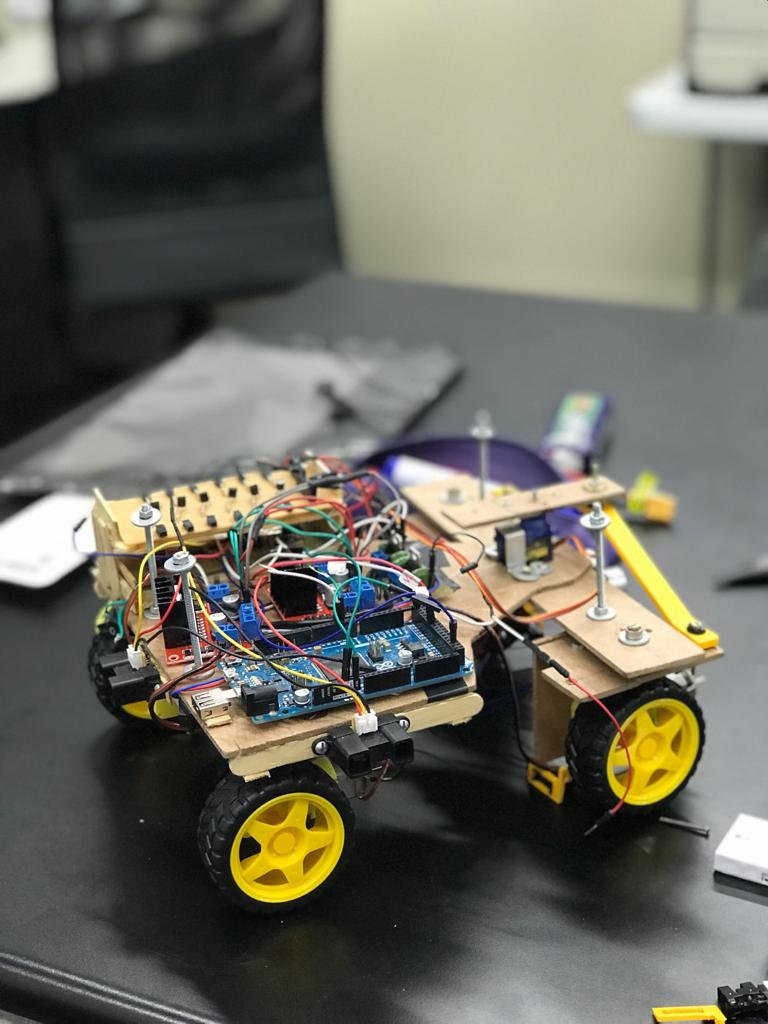
\includegraphics[width=0.5\textwidth]{02_desenvolvimento/04_EC_Fig_CarrinhoFoto.jpeg}
		\caption{Protótipo do veículo autônomo.}
		\label{fig:4ec-carrinhofoto}
	\end{figure}
	
	As Tabelas \ref{tab:4ec-carrinholimacoes1} e \ref{tab:4ec-carrinholimacoes2} apresentam as restrições definidas para a simulação, quando as variáveis de controle são $v$ e $\phi$ ou $\dot{v}$ e $\dot{\phi}$, respectivamente.
	
	\begin{table}[H]
		\centering
		\caption{Limites para as variáveis de controle $v$ e $\phi$.}
		\label{tab:4ec-carrinholimacoes1}
		\begin{tabular}{l|l|l} \toprule
			{Variável} & {Mínimo} & {Máximo}\\ \midrule
			{$v$} & {-0,1 \si{m/s}} & {0,1 \si{m/s}} \\
			{$\phi$} & {-0,5 \si{rad/s}} & {0,5 \si{rad/s}} \\
			\bottomrule
		\end{tabular}
	\end{table}

	\begin{table}[H]
		\centering
		\caption{Restrições ao controle exercido por meio das variáveis $\dot{v}$ e $\dot{\phi}$.}
		\label{tab:4ec-carrinholimacoes2}
		\begin{tabular}{l|l|l} \toprule
			{Variável} & {Mínimo} & {Máximo}\\ \midrule
			{$\dot{v}$} & {-0,1 \si{m/s}} & {0,1 \si{m/s}} \\
			{$\dot{\phi}$} & {-0,5 \si{rad/s}} & {0,5 \si{rad/s}} \\
			\bottomrule
		\end{tabular}
	\end{table}
	
	\item \underline{A função de recompensa:}
	
	Para os casos em que se deseja apenas chegar ao alvo, independentemente da orientação do robô no local, a função de recompensa é:
	
%	\begin{equation}\label{eq:4ec-carrinhorecompsemang}
%	r(t)=
%	\begin{cases}
%	-10000\,\text{caso o veículo ultrapasse dos limites estabelecidos na Tabela \ref{tab:4ec-carrinholimvariaveis} \\
%	2000\,\text{se $d\le R$, onde R é a tolerância.}\\
%	-d\,,\qquad\text{caso contrário. Onde $d$ é a distância entre o robô e o alvo.}
%	\end{cases}
%	\end{equation}
%	
%	\begin{equation}
%		\begin{cases}
%		-10000\\
%		2000\\
%		-d
%		\end{cases}
%	\end{equation}
	
	\begin{align}\label{eq:4ec-carrinhorecompsemang}
	\begin{split}
	r(t)=\begin{cases}
	-1000\,,\hspace{2cm} O(t)\notin\mathcal{S}_O\\
	2000\,,\hspace{2.5cm} d\le R\\
	-d
	\end{cases}
	\end{split}
	\end{align}
	
	Quando deseja-se considerar a orientação do robô na posição do alvo, a função de recompensa será:
	
	\begin{align}\label{eq:4ec-carrinhorecompcomang}
	\begin{split}
	r(t)=\begin{cases}
	-1000\,,\hspace{2cm} O(t)\notin\mathcal{S}_O\\
	2000\cdot|\theta_{ref}-\theta|\,,\hspace{0.6cm} d\le R\\
	-d
	\end{cases}
	\end{split}
	\end{align}
	
	Nota-se que $\mathcal{S}_O$ representa o espaço de observação, isto é, o conjunto de valores das variáveis de estado que não causam o término do episódio, conforme estabelecido na Tabela \ref{tab:4ec-carrinholimvariaveis}.
	
	\item \underline{Os critérios de término do episódio:}
	
	Naturalmente, deve haver um tempo limite para cada simulação. Além disso, caso o veículo não obedeça os limites estabelecidos na Tabela \ref{tab:4ec-carrinholimvariaveis} ou atinja o alvo, dentro da tolerância estabelecida, o episódio de simulação é terminado automaticamente. 
	
\end{enumerate}

A partir dessas características, os métodos da biblioteca Gym (Capítulo \ref{ssec:2gym-openaigym}) foram implementados, incluindo a função \textit{render}, que permite visualizar a simulação em tempo real, através de um vídeo.

\begin{figure}[H]
	\centering
	\includegraphics[width=0.6\textwidth]{02_desenvolvimento/04_EC_Fig_CarrinhoRender.png}
	\caption{\textit{Frame} do vídeo em um episódio de simulação.}
	\label{fig:4ec-carrinhorender}
\end{figure}

Existe uma particularidade na aplicação da PG neste problema: cada indivíduo deve produzir dois valores de controle. Nos casos anteriores abordados, havia uma única ação, o que tornou a aplicação da PG imediata, já que cada árvore produz um único resultado numérico.

Para contornar este problema, é utilizada a programação genética \textit{multigênica}, onde cada indivíduo é composto de duas árvores: uma responsável pelo controle de $v$ (ou $\dot{v}$) e outra para a variável $\phi$ (ou $\dot{\phi}$). As operações genéticas são aplicadas em cada árvore do indivíduo. Especificamente, para a operação de cruzamento, a recombinação ocorre entre árvores que controlam a mesma variável.

Para que os valores de controle produzidos pelos indivíduos respeitem os limites estabelecidos nas Tabelas \ref{tab:4ec-carrinholimacoes1} e \ref{tab:4ec-carrinholimacoes2}, o valor resultante da avaliação da árvore é truncado com a função \textit{clip} (Figura \ref{fig:4ec-pendulumclip}).

Algumas situações específicas relacionadas a este problema foram abordadas, em ordem de complexidade.

\begin{enumerate}[label=Problema \arabic*)]
	\item A partir de uma posição inicial \textbf{fixa}, chegar ao alvo com \textbf{qualquer} orientação ao controlar as entradas $v$ e $\phi$. Admite-se a possibilidade de variação instantânea dessas variáveis.
	\item A partir de uma posição inicial \textbf{fixa}, chegar ao alvo com uma orientação \textbf{definida} ao controlar as entradas $v$ e $\phi$. Admite-se a possibilidade de variação instantânea dessas variáveis.
	\item A partir de uma posição inicial \textbf{aleatória}, chegar ao alvo com \textbf{qualquer} orientação ao controlar as entradas $\dot{v}$ e $\dot{\phi}$.
	\item A partir de uma posição inicial \textbf{aleatória}, chegar ao alvo com uma orientação \textbf{definida} ao controlar as entradas $\dot{v}$ e $\dot{\phi}$.
\end{enumerate}

Para os problemas 3 e 4, a aleatoriedade da posição inicial é estabelecida a partir dos parâmetros $\delta_x$, $\delta_y$ e $\delta_\theta$, apresentados na Figura \ref{fig:4ec-carrinhovisaogeral}.

\subsubsection{Problema 1}\label{sssec:4ec-carrinhoprob1}

Neste caso, não há um objetivo associado à orientação do veículo e a pose inicial é fixa. Portanto, não é necessário que a avaliação de um indivíduo ocorra em vários episódios. A visão geral do problema pode ser vista na Figura \ref{fig:4ec-carrinhoprob1visaogeral}.

\begin{figure}[H]
	\centering
	\includegraphics[width=0.8\textwidth]{02_desenvolvimento/04_EC_Fig_CarrinhoProb1VisaoGeral.pdf}
	\caption{Primeira situação.}
	\label{fig:4ec-carrinhoprob1visaogeral}
\end{figure}

Os parâmetros utilizados para a programação genética são apresentados na Tabela \ref{tab:4ec-carrinhoprob1parampg}.

\begin{table}[H]
	\centering
	\begin{tabular}{l|l} \toprule
		{Parâmetro} & {Valor} \\ \midrule
		{Tamanho da População} & {500} \\
		{Probabilidade de Cruzamento} & {0,75} \\
		{Probabilidade de Mutação} & {0,05} \\
		{Número de Gerações} & {15} \\
		{Número de Entradas} & {6} \\
		{Faixa para Constante Efêmera} & {(-1, 1)} \\
		{Número de Simulações} & {1} \\
		{Tamanho do Campeonato de Aptidão} & {6} \\
		{Operações} & {$+,\,-,\,\times,\,\div,\,\sqrt{},\,\sin,\,>$, sgn} \\
		{Comprimento Mínimo e Máximo de Inicialização} & {(2, 5)} \\
		{Comprimento Máximo de Mutação} & {7} \\
		{Limite de Comprimento dos Indivíduos} & {17} \\
		\bottomrule
	\end{tabular}
	\caption{Parâmetros utilizados para o problema 1 do carro robô.}\label{tab:4ec-carrinhoprob1parampg}
\end{table}

Em conformidade com a abordagem utilizada até o momento, a aptidão é calculada a partir de uma função de recompensa (Equação \ref{eq:4ec-carrinhorecompsemang}).

\begin{align}\label{eq:4ec-carrinhoprob1aptidao}
\begin{split}
&A(t) = r(t),\,\,\forall t<T\\\\
&A_{tot} = \sum_{t=0}^{T} r(t),\,\qquad r(t) =
\begin{cases}
-1000\,,\qquad O(t)\notin\mathcal{S}_O\\
2000\,,\qquad\hspace{1.25em} d\le R\\
-d
\end{cases} \\
&\bar{A} = A_{tot}
\end{split}
\end{align}

Os gráficos relacionados à aptidão dos indivíduos, ao longo das gerações, podem ser visto nas Figuras \ref{fig:4ec-carrinhoprob1aptger} e \ref{fig:4ec-carrinhoprob1apthist}. As aptidões positivas indicam, necessariamente, que o indivíduo chegou ao local alvo. Dentre esses, os que alcançam o objetivo no menor tempo devem apresentar um desempenho melhor.

\begin{figure}[H]
	\centering
	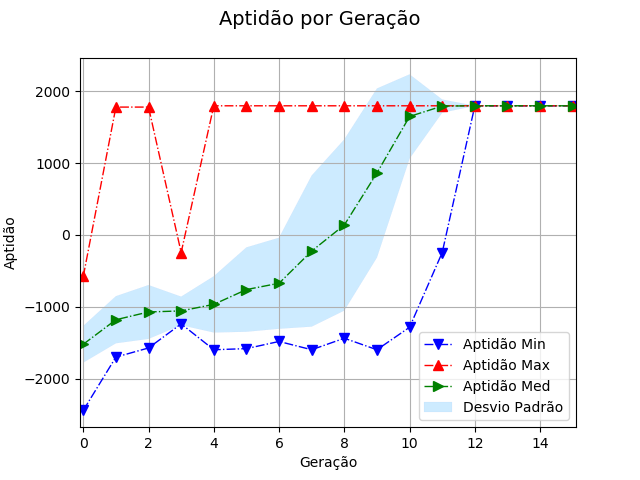
\includegraphics[width=0.8\textwidth]{02_desenvolvimento/04_EC_Fig_CarrinhoProb1AptGer.png}
	\caption{Aptidão dos indivíduos.}
	\label{fig:4ec-carrinhoprob1aptger}
\end{figure}

É possível perceber, na Figura \ref{fig:4ec-carrinhoprob1aptger}, que na terceira geração alguns indivíduos já são capazes de alcançar o local alvo.

\begin{figure}[H]
	\centering
	\includegraphics[width=0.8\textwidth]{02_desenvolvimento/04_EC_Fig_CarrinhoProb1AptHist.png}
	\caption{Histograma das aptidões.}
	\label{fig:4ec-carrinhoprob1apthist}
\end{figure}

O indivíduo que obteve melhor desempenho pode ser visto na Figura \ref{fig:4ec-carrinhoprob1arvore}. A trajetória deste indivíduo é apresentada na Figuras \ref{fig:4ec-carrinhoprob1trajgraf}.

\begin{figure}[H]
	\centering
	\includegraphics[width=0.99\textwidth]{02_desenvolvimento/04_EC_Fig_CarrinhoProb1Arvores.png}
	\caption{Árvores de controle do melhor indivíduo encontrado.}
	\label{fig:4ec-carrinhoprob1arvore}
\end{figure}

%\begin{figure}[H]
%	\centering
%	\includegraphics[width=0.8\textwidth]{02_desenvolvimento/04_EC_Fig_CarrinhoProb1TrajRender.pdf}
%	\caption{Trajetória exibida pelo melhor indivíduo.}
%	\label{fig:4ec-carrinhoprob1trajrender}
%\end{figure}

\begin{figure}[H]
	\centering
	\includegraphics[width=0.8\textwidth]{02_desenvolvimento/04_EC_Fig_CarrinhoProb1TrajGraf.png}
	\caption{Trajetória do indivíduo de melhor desempenho. As setas indicam a orientação do veículo ao longo da trajetória.}
	\label{fig:4ec-carrinhoprob1trajgraf}
\end{figure}

%É possível observar que a árvore que controla a velocidade gera sempre uma constante que, ao ser fornecida como entrada para a função \textit{clip}, produz a maior taxa de variação da posição em relação ao tempo permitida. Consequentemente, o indivíduo chega mais rápido ao local alvo. Este fenômeno pode ser observado na Figura \ref{fig:4ec-carrinhoprob1vargraf}.

A Figura \ref{fig:4ec-carrinhoprob1vargraf} ilustra o controle exercido pelo melhor indivíduo durante a simulação.

\begin{figure}[H]
	\centering
	\includegraphics[width=0.8\textwidth]{02_desenvolvimento/04_EC_Fig_CarrinhoProb1VarGraf.png}
	\caption{Saída das funções de controle ao longo da simulação.}
	\label{fig:4ec-carrinhoprob1vargraf}
\end{figure}

Os dados relativos à execução do algoritmo podem ser vistos na Tabela \ref{tab:4ec-carrinhoprob1custocomp}.

\begin{table}[H]
	\centering
	\begin{tabular}{l|l} \toprule
		% {} & {\textbf{PG}} \\ \midrule
		{{Tempo de execução (h:m:s)}} & {00:34:26} \\\midrule
		{{Passos de simulação}} & {5062016} \\\midrule
		{{Número de episódios}} & {6503} \\
		\bottomrule
	\end{tabular}
	\caption{Problema 1 - custo computacional.}\label{tab:4ec-carrinhoprob1custocomp}
\end{table}

Para este problema inicial, fica claro que a programação genética multigênica pode gerar um indivíduo capaz de guiar o veículo até o alvo.

\subsubsection{Problema 2}\label{sssec:4ec-carrinhoprob2}

Neste problema é tratado o caso em que o robô deve chegar ao lugar desejado com uma determinada orientação. A única diferença na implementação do algoritmo, para este caso, reside na mudança da função de recompensa (Equação \ref{eq:4ec-carrinhorecompcomang}). Será considerado um ângulo desejado igual ao de partida, isto é, zero.

\begin{figure}[H]
	\centering
	\includegraphics[width=0.8\textwidth]{02_desenvolvimento/04_EC_Fig_CarrinhoProb2VisaoGeral.pdf}
	\caption{Visão geral do problema 2.}
	\label{fig:4ec-carrinhoprob2visaogeral}
\end{figure}

A função de recompensa deve levar em conta o ângulo de orientação, quando o robô chega ao alvo. Portanto, utiliza-se a Equação \ref{eq:4ec-carrinhorecompcomang}, com $\theta_{ref}=0$. A aptidão de um indivíduo é tal como descrita na Equação \ref{eq:4ec-carrinhoprob2aptidao}

\begin{align}\label{eq:4ec-carrinhoprob2aptidao}
\begin{split}
&A(t) = r(t),\,\forall t<T\\\\
&A_{tot} = \sum_{t=0}^{T} r(t),\,\qquad r(t) =
\begin{cases}
-1000\,,\qquad\hspace{1em} O(t)\notin\mathcal{S}_O\\
2000\cdot|\theta|\,,\qquad\hspace{0.45em} d\le R\\
-d\qquad
\end{cases} \\
&\bar{A} = A_{tot}
\end{split}
\end{align}

Foram utilizados os mesmos parâmetros do caso anterior (Tabela \ref{tab:4ec-carrinhoprob1parampg}) para a obtenção dos resultados a seguir:

\begin{figure}[H]
	\centering
	\includegraphics[width=0.8\textwidth]{02_desenvolvimento/04_EC_Fig_CarrinhoProb2AptGer.png}
	\caption{Aptidão dos indivíduos.}
	\label{fig:4ec-carrinhoprob2aptger}
\end{figure}

\begin{figure}[H]
	\centering
	\includegraphics[width=0.8\textwidth]{02_desenvolvimento/04_EC_Fig_CarrinhoProb2AptHist.png}
	\caption{Histograma das aptidões.}
	\label{fig:4ec-carrinhoprob2apthist}
\end{figure}

\begin{figure}[H]
	\centering
	\includegraphics[width=\textwidth]{02_desenvolvimento/04_EC_Fig_CarrinhoProb2Arvores.png}
	\caption{Indivíduo que obteve melhor desempenho.}
	\label{fig:4ec-carrinhoprob2arvores}
\end{figure}

%\begin{figure}[H]
%	\centering
%	\includegraphics[width=0.8\textwidth]{02_desenvolvimento/04_EC_Fig_CarrinhoProb2TrajRender.pdf}
%	\caption{Trajetória do indivíduo da Figura \ref{fig:4ec-carrinhoprob2arvores}.}
%	\label{fig:4ec-carrinhoprob2trajrender}
%\end{figure}

É possível perceber nas Figuras \ref{fig:4ec-carrinhoprob2trajgraf} e \ref{fig:4ec-carrinhoprob2vargraf} que o indivíduo, quando o veículo está próximo ao objetivo, gera valores para $v$ e $\phi$ que alternam entre o mínimo e máximo permitidos, causando uma mudança brusca na orientação do veículo sem grandes alterações na sua posição.

\begin{figure}[H]
	\centering
	\includegraphics[width=0.8\textwidth]{02_desenvolvimento/04_EC_Fig_CarrinhoProb2TrajGraf.png}
	\caption{Trajetória do indivíduo da Figura \ref{fig:4ec-carrinhoprob2arvores}.}
	\label{fig:4ec-carrinhoprob2trajgraf}
\end{figure}

\begin{figure}[H]
	\centering
	\includegraphics[width=0.8\textwidth]{02_desenvolvimento/04_EC_Fig_CarrinhoProb2VarGraf.png}
	\caption{Funções temporais geradas.}
	\label{fig:4ec-carrinhoprob2vargraf}
\end{figure}

O custo computacional, associado à execução do algoritmo, pode ser visto na Tabela \ref{tab:4ec-carrinhoprob2custocomp}.

\begin{table}[H]
	\centering
	\begin{tabular}{l|l} \toprule
		{{Tempo de execução (h:m:s)}} & {00:35:43} \\\midrule
		{{Passos de simulação}} & {5290938} \\\midrule
		{{Número de episódios}} & {6452} \\
		\bottomrule
	\end{tabular}
	\caption{Problema 2: custo computacional.}\label{tab:4ec-carrinhoprob2custocomp}
\end{table}

Na Figura \ref{fig:4ec-carrinhoprob2trajgraf} é possível notar que o objetivo proposto foi alcançado.

\subsubsection{Problema 3}\label{sssec:4ec-carrinhoprob3}

Neste problema é considerado o caso em que a pose inicial do robô é aleatória, tornando-o semelhante aos problemas iniciais da biblioteca Gym. Não há um objetivo associado à orientação do robô, ou seja, a função de recompensa utilizada é a Equação \ref{eq:4ec-carrinhorecompsemang}. O controle é exercido por meio das variáveis $\dot{v}$ e $\dot{\phi}$, portanto, a simulação possui uma maior conformidade com a situação real.

Devido à aleatoriedade da pose inicial, é necessário aumentar o número de simulações para cada indivíduo, o que garante que os indivíduos selecionados tenham uma boa capacidade de generalização. A Figura \ref{fig:4ec-carrinhoprob3visaogeral} mostra o problema proposto.

\begin{figure}[H]
	\centering
	\includegraphics[width=0.85\textwidth]{02_desenvolvimento/04_EC_Fig_CarrinhoProb3VisaoGeral.pdf}
	\caption{Visão geral do problema 3.}
	\label{fig:4ec-carrinhoprob3visaogeral}
\end{figure}

Pode-se perceber na Figura \ref{fig:4ec-carrinhoprob3visaogeral} os valores iniciais possíveis para a posição e orientação do robô.

Os parâmetros da programação genética são os mesmos da Tabela \ref{tab:4ec-carrinhoprob1parampg}, com exceção do \textbf{número de simulações} definido como \textbf{30} e o \textbf{número de gerações, 30}. 

A função de aptidão deve levar em conta todos os episódios de simulação do indivíduo:, conforme indica a Equação \ref{eq:4ec-carrinhoprob3aptidao}.

\begin{align}\label{eq:4ec-carrinhoprob3aptidao}
	\begin{split}
	&A(t) = r(t),\,\forall t<T\\\\
	&A_{tot}^{ep} = \sum_{t=0}^{T} r(t),\,\qquad r(t) =  
		\begin{cases}
		-1000\,,\qquad O(t)\notin\mathcal{S}_O\\
		2000\,,\qquad\hspace{1.25em} d\le R\\
		-d
		\end{cases}	\\
	&\bar{A} = \sum_{ep=1}^{40}A_{tot}^{ep}
	\end{split}
\end{align}

As Figuras \ref{fig:4ec-carrinhoprob3aptger} e \ref{fig:4ec-carrinhoprob3apthist} mostram as estatísticas relacionadas à aptidão da população. 

% Independe do modo que a aptidao é calculada, apenas do que é obtido de forma automatica. Independe do Q learning, independe da forma de obtencao da recompensa. Nao pode ser confundido com a forma 

\begin{figure}[H]
	\centering
	\includegraphics[width=0.8\textwidth]{02_desenvolvimento/04_EC_Fig_CarrinhoProb3AptGer.png}
	\caption{Aptidão da população ao longo de 30 gerações.}
	\label{fig:4ec-carrinhoprob3aptger}
\end{figure}

\begin{figure}[H]
	\centering
	\includegraphics[width=0.8\textwidth]{02_desenvolvimento/04_EC_Fig_CarrinhoProb3AptHist.png}
	\caption{Histograma de aptidões.}
	\label{fig:4ec-carrinhoprob3apthist}
\end{figure}

O melhor indivíduo encontrado pode ser visto na Figura \ref{fig:4ec-carrinhoprob3arvores}.

\begin{figure}[H]
	\centering
	\includegraphics[width=\textwidth]{02_desenvolvimento/04_EC_Fig_CarrinhoProb3Arvores.png}
	\caption{Árvores de controle do indivíduo que apresentou melhor desempenho.}
	\label{fig:4ec-carrinhoprob3arvores}
\end{figure}

Algumas trajetórias exibidas pelo indivíduo da Figura \ref{fig:4ec-carrinhoprob3arvores}, com os valores extremos da condição inicial, podem ser vistas nas Figuras \ref{fig:4ec-carrinhoprob3trajgraf1}, \ref{fig:4ec-carrinhoprob3trajgraf2} e \ref{fig:4ec-carrinhoprob3trajgraf3}. Na parte superior esquerda de cada figura, é possível observar a aptidão obtida pelo agente.

\begin{figure}[H]
	\centering
	\includegraphics[width=0.8\textwidth]{02_desenvolvimento/04_EC_Fig_CarrinhoProb3TrajGraf1.png}
	\caption{Trajetórias exibidas pelo melhor indivíduo com ângulo de orientação inicial igual a $0$. As coordenadas $X_0$ e $Y_0$ são os valores extremos possíveis ($0.15$ e $0.20$) e o valor médio ($0.20$).}
	\label{fig:4ec-carrinhoprob3trajgraf1}
\end{figure}

Considerando os mesmos valores de $X_0$ e $Y_0$ iniciais, porém com o ângulo de orientação inicial igual a $\ang{30}$ e $\ang{-30}$, foram obtidos os gráficos da Figura \ref{fig:4ec-carrinhoprob3trajgraf2} e \ref{fig:4ec-carrinhoprob3trajgraf3}, respectivamente.

\begin{figure}[H]
	\centering
	\includegraphics[width=0.8\textwidth]{02_desenvolvimento/04_EC_Fig_CarrinhoProb3TrajGraf2.png}
	\caption{$\theta_0=\ang{30}$}
	\label{fig:4ec-carrinhoprob3trajgraf2}
\end{figure}

\begin{figure}[H]
	\centering
	\includegraphics[width=0.8\textwidth]{02_desenvolvimento/04_EC_Fig_CarrinhoProb3TrajGraf3.png}
	\caption{$\theta_0=\ang{-30}$}
	\label{fig:4ec-carrinhoprob3trajgraf3}
\end{figure}

Observa-se que as aptidões positivas indicam que o robô chegou ao local alvo (com tolerância de $\SI{3}{cm}$).

%Algumas condições iniciais causam o robô a realizar um movimento de \textit{zig-zag} próximo ao alvo, porém nem sempre o objetivo final é atingido, com a devida tolerância.

Para verificar a taxa de sucesso do robô em atingir o local alvo, foram consideradas as situações iniciais formadas pela combinação de 10 valores igualmente espaçados para cada variável ($X_0$, $Y_0$ e $\theta_0$), dentre os limites estabelecidos, totalizando \textbf{1000 simulações} com condições inicias diferentes.

O alvo foi alcançado em $770$ episódios, indicando uma taxa de sucesso aproximada de $77\%$. O custo computacional pode ser observado na Tabela \ref{tab:4ec-carrinhoprob3custocomp}.

\begin{table}[H]
	\centering
	\begin{tabular}{l|l} \toprule
		{{Tempo de execução (h:m:s)}} & {37:14:08} \\\midrule
		{{Passos de simulação}} & {333557152} \\\midrule
		{{Número de episódios}} & {374760} \\
		\bottomrule
	\end{tabular}
	\caption{Custo computacional para o problema 3.}\label{tab:4ec-carrinhoprob3custocomp}
\end{table}

\subsubsection{Problema 4}\label{sssec:4ec-carrinhoprob4}

O último problema se assemelha ao caso anterior, entretanto, deseja-se também que o robô atinja uma determinada orientação ao fim da trajetória. Isto é, a única diferença reside na função de recompensa, onde será utilizada a Equação \ref{eq:4ec-carrinhorecompcomang}, para o cálculo da aptidão, conforme indica a Equação \ref{eq:4ec-carrinhoprob4aptidao}.

\begin{align}\label{eq:4ec-carrinhoprob4aptidao}
	\begin{split}
		&A(t) = r(t),\,\forall t<T\\\\
		&A_{tot}^{ep} = \sum_{t=0}^{T} r(t),\,\qquad r(t) =  
			\begin{cases}
			-1000\,,\qquad\hspace{0.28em} O(t)\notin\mathcal{S}_O\\
			2000\cdot |\theta|\,,\qquad d\le R\\
			-d
			\end{cases}	\\
		&\bar{A} = \sum_{ep=1}^{40}A_{tot}^{ep}
	\end{split}
\end{align}

A situação proposta pelo problema 4 está esquematizada na Figura \ref{fig:4ec-carrinhoprob4visaogeral}.

\begin{figure}[H]
	\centering
	\includegraphics[width=0.8\textwidth]{02_desenvolvimento/04_EC_Fig_CarrinhoProb4VisaoGeral.pdf}
	\caption{Visão geral do problema 4.}
	\label{fig:4ec-carrinhoprob4visaogeral}
\end{figure}

Os resultados obtidos podem ser verificados nas Figuras \ref{fig:4ec-carrinhoprob4aptger} a \ref{fig:4ec-carrinhoprob4trajgraf1}.

\begin{figure}[H]
	\centering
	\includegraphics[width=\textwidth]{02_desenvolvimento/04_EC_Fig_CarrinhoProb4AptGer.png}
	\caption{Aptidão ao longo das gerações para o problema 3.}
	\label{fig:4ec-carrinhoprob4aptger}
\end{figure}

\begin{figure}[H]
	\centering
	\includegraphics[width=0.8\textwidth]{02_desenvolvimento/04_EC_Fig_CarrinhoProb4AptHist.png}
	\caption{Histograma das aptidões.}
	\label{fig:4ec-carrinhoprob4apthist}
\end{figure}

\begin{figure}[H]
	\centering
	\includegraphics[width=\textwidth]{02_desenvolvimento/04_EC_Fig_CarrinhoProb4Arvores.png}
	\caption{Árvores de controle do indivíduo de melhor desempenho encontrado.}
	\label{fig:4ec-carrinhoprob4arvores}
\end{figure}

\begin{figure}[H]
	\centering
	\includegraphics[width=0.8\textwidth]{02_desenvolvimento/04_EC_Fig_CarrinhoProb4TrajGraf1.png}
	\caption{Trajetórias exibidas pelo melhor indivíduo com ângulo de orientação igual a $0$. As coordenadas $X_0$ e $Y_0$ são os valores extremos ($0.15$ e $0.20$) e o valor médio ($0.20$).}
	\label{fig:4ec-carrinhoprob4trajgraf1}
\end{figure}

Novamente consideramos os mesmos $X_0$ e $Y_0$, com diferentes ângulos de orientação inicial. As Figuras \ref{fig:4ec-carrinhoprob3trajgraf2} e \ref{fig:4ec-carrinhoprob4trajgraf3}, mostram os resultados obtidos.

\begin{figure}[H]
	\centering
	\includegraphics[width=0.8\textwidth]{02_desenvolvimento/04_EC_Fig_CarrinhoProb4TrajGraf2.png}
	\caption{$\theta_0=\ang{30}$}
	\label{fig:4ec-carrinhoprob4trajgraf2}
\end{figure}

\begin{figure}[H]
	\centering
	\includegraphics[width=0.8\textwidth]{02_desenvolvimento/04_EC_Fig_CarrinhoProb4TrajGraf3.png}
	\caption{$\theta_0=\ang{-30}$}
	\label{fig:4ec-carrinhoprob4trajgraf3}
\end{figure}

Ao considerar, de forma semelhante ao problema anterior, 1000 simulações com condições iniciais distintas, a taxa de sucesso obtido foi de $51.9\%$. Como o problema em questão formula um objetivo ao redor do ângulo de chegada, foi obtida a média dos ângulos de orientação do carro. O valor encontrado foi 20\degree.

\begin{table}[H]
	\centering
	\begin{tabular}{l|l} \toprule
		{} & {{PG}} \\ \midrule
		{{Tempo de execução (h:m:s)}} & {33:47:56} \\
		{{Passos de simulação}} & {289651497} \\
		{{Número de episódios}} & {377340} \\
		\bottomrule
	\end{tabular}
	\caption{Problema 4: custo computacional.}\label{tab:4ec-carrinhoprob4custocomp}
\end{table}
